\documentclass[final,11pt]{article}
\usepackage[utf8]{inputenc}
\usepackage[T1]{fontenc}
\usepackage[english]{babel}
\usepackage{graphicx}
\graphicspath{{img/}}
\usepackage{appendix}[titletoc]
\usepackage{algorithm2e}
\usepackage{enumitem}
\usepackage{caption}
\usepackage{bbm}
\usepackage{pgfplots}
\usepackage{amsmath}
\usepackage{amsthm}
\usepackage{amssymb}
\usepackage{hyperref}
\usepackage{array}
\usepackage{tikz}
\usepackage{float}
\usepackage{booktabs}
\usepackage{multirow}
\usepackage[square,numbers]{natbib}
\bibliographystyle{plainnat}
\usepackage[margin=1in]{geometry}

\hypersetup{
    pdftitle={Maximizing Confidentiality in Encrypted Search\\
    Through Entropy Optimization
},                            % title
    pdfauthor={Alexander Towell},               % author
    pdfsubject={computer science},              % subject of the document
    pdfkeywords={
        encrypted search,
        homomorphic encryption,
        known-plaintext attacks,
        oblivious searches,
        information retrieval,
        information security,
        resilience engineering
        maximum likelihood estimation,
        obfuscation,
        query privacy},                         % keywords
    colorlinks=false,                           % false: boxed links; true: colored links
    citecolor=green,                            % color of links to bibliography
    filecolor=magenta,                          % color of file links
    urlcolor=green                              % color of external links
}

% Random variable notation from rv.tex
\newcommand{\hrs}[1][]{%
   \ifthenelse{ \equal{#1}{} }
      {\ensuremath{\vec{\check{d}}}}
      {\ensuremath{\vec{\check{d}_{#1}}}}
}
\newcommand{\rvhrs}[1][]{%
   \ifthenelse{ \equal{#1}{} }
      {\ensuremath{\rv{\vec{\check{D}}}}}
      {\ensuremath{\rv{\vec{\check{D}_{#1}}}}}
}
\newcommand{\rs}[1][]{%
   \ifthenelse{ \equal{#1}{} }
      {\ensuremath{\vec{d}}}
      {\ensuremath{\vec{d_{#1}}}}
}
\newcommand{\rvrs}[1][]{%
   \ifthenelse{ \equal{#1}{} }
      {\ensuremath{\rv{\vec{D}}}}
      {\ensuremath{\rv{\vec{D_{#1}}}}}
}
\newcommand{\hqb}[1][]{%
   \ifthenelse{ \equal{#1}{} }
      {\ensuremath{\vec{\check{x}}}}
      {\ensuremath{\vec{\check{x}_{#1}}}}
}
\newcommand{\rvhqb}[1][]{%
   \ifthenelse{ \equal{#1}{} }
      {\ensuremath{\rv{\vec{\check{X}}}}}
      {\ensuremath{\rv{\vec{\check{X}_{#1}}}}}
}
\newcommand{\qb}[1][]{%
   \ifthenelse{ \equal{#1}{} }
      {\ensuremath{\vec{x}}}
      {\ensuremath{\vec{x_{#1}}}}
}
\newcommand{\rvqb}[1][]{%
   \ifthenelse{ \equal{#1}{} }
      {\ensuremath{\rv{\vec{X}}}}
      {\ensuremath{\rv{\vec{X_{#1}}}}}
}
\newcommand{\ts}[1][]{%
   \ifthenelse{ \equal{#1}{} }
      {\ensuremath{t}}
      {\ensuremath{t_{#1}}}
}
\newcommand{\rvts}[1][]{%
   \ifthenelse{ \equal{#1}{} }
      {\ensuremath{\rv{T}}}
      {\ensuremath{\rv{T_{#1}}}}
}
\newcommand{\hts}[1][]{%
   \ifthenelse{ \equal{#1}{} }
      {\ensuremath{\check{t}}}
      {\ensuremath{\check{t}_{#1}}}
}
\newcommand{\rvhts}[1][]{%
   \ifthenelse{ \equal{#1}{} }
      {\ensuremath{\rv{\check{T}}}}
      {\ensuremath{\rv{\check{T}_{#1}}}}
}
\newcommand{\hsa}[1][]{%
   \ifthenelse{ \equal{#1}{} }
      {\ensuremath{\check{a}}}
      {\ensuremath{\check{a}_{#1}}}
}
\newcommand{\rvhsa}[1][]{%
   \ifthenelse{ \equal{#1}{} }
      {\ensuremath{\rv{\check{A}}}}
      {\ensuremath{\rv{\check{A}_{#1}}}}
}
\newcommand{\sa}[1][]{%
   \ifthenelse{ \equal{#1}{} }
      {\ensuremath{a}}
      {\ensuremath{a_{#1}}}
}
\newcommand{\rvsa}[1][]{%
   \ifthenelse{ \equal{#1}{} }
      {\ensuremath{\rv{A}}}
      {\ensuremath{\rv{A_{#1}}}}
}
\newcommand{\htup}[1][]{%
   \ifthenelse{ \equal{#1}{} }
      {\ensuremath{\vec{\check{q}}}}
      {\ensuremath{\vec{\check{q}_{#1}}}}
}
\newcommand{\rvhtup}[1][]{%
   \ifthenelse{ \equal{#1}{} }
      {\ensuremath{\rv{\vec{\check{Q}}}}}
      {\ensuremath{\rv{\vec{\check{Q}_{#1}}}}}
}
\newcommand{\tup}[1][]{%
   \ifthenelse{ \equal{#1}{} }
      {\ensuremath{\vec{q}}}
      {\ensuremath{\vec{q_{#1}}}}
}
\newcommand{\rvtup}[1][]{%
   \ifthenelse{ \equal{#1}{} }
      {\ensuremath{\rv{\vec{Q}}}}
      {\ensuremath{\rv{\vec{Q_{#1}}}}}
}

% Definitions from defs.tex
\SetKwInOut{KwIn}{input}
\SetKwInOut{KwOut}{output}
\SetKwInOut{parameters}{params}

\SetKwFunction{BL}{BL}
\SetKwFunction{containsfn}{contains}
\SetKwFunction{diffn}{difference}
\SetKwFunction{andfn}{and}
\SetKwFunction{orfn}{or}
\SetKwFunction{notfn}{not}
\SetKwFunction{PowerSetFn}{powerset}
\SetKwFunction{perfecthash}{ph}
\SetKwFunction{cryptohash}{ch}
\SetKwFunction{encrypt}{encrypt}
\SetKwFunction{Decrypt}{decrypt}
\SetKwFunction{Encrypt}{Encrypt}
\SetKwFunction{Dim}{dim}
\SetKwFunction{ph}{ph}
\SetKwFunction{ro}{h$^*$}
\SetKwFunction{hash}{h}
\SetKwFunction{HiddenQueryGenerator}{hidden\_query\_generator}
\SetKwFunction{HiddenQueryNoiseDecorator}{hidden\_query\_noise\_decorator}
\SetKwFunction{sampler}{obfuscated\_time\_series\_sampler}
\SetKwFunction{Compress}{compress}
\SetKwFunction{Powerset}{powerset}
\SetKwFunction{Decompress}{decompress}
\SetKwFunction{Encode}{encode}
\SetKwFunction{Decode}{decode}
\SetKwFunction{Doc}{doc}
\SetKwFunction{Ref}{ref}
\SetKwFunction{SecureIndexMaker}{secure\_index\_maker}
\SetKwFunction{SecureIndex}{secure\_index}
\SetKwFunction{HiddenQueryMapper}{hidden\_query\_mapper}
\SetKwFunction{substitutions}{substitutions}
\SetKwFunction{Concat}{concat}

\SetKwFunction{MakeSecureIndex}{make\_secure\_index}

\newcommand{\catop}{{+\!\!+}}
\newcommand{\derivative}[1]{\frac {\mathrm{d}}{\mathrm{d}#1}}
\newcommand{\pderivative}[1]{\frac {\mathrm{\partial}}{\mathrm{\partial}#1}}
\newcommand{\rv}[1]{\mathrm{#1}}
\newcommand{\likelihood}{\mathcal{L}}
\newcommand{\entropy}{\operatorname{\mathcal{H}}}
\newcommand{\info}{\operatorname{\mathcal{I}}}
\newcommand{\cdf}{\operatorname{F}}
\newcommand{\pdf}{\operatorname{f}}
\newcommand{\haz}{\operatorname{h}}
\newcommand{\srv}{\operatorname{R}}
\newcommand{\pmf}{\operatorname{p}}
\newcommand{\prob}{\Pr}
\newcommand{\kth}{$k^{\text{th }}$}
\newcommand{\ith}{$i^{\text{th }}$}
\newcommand{\jth}{$j^{\text{th }}$}
\newcommand{\nth}{$n^{\text{th }}$}
\newcommand{\rth}{$r^{\text{th }}$}
\newcommand{\pth}{$p^{\text{th }}$}
\newcommand{\mvndist}{\operatorname{\rm{MVN}}}
\newcommand{\expdist}{\operatorname{\rm{EXP}}}
\newcommand{\zipf}{\operatorname{\rm{Zipf}}}
\newcommand{\geodist}{\operatorname{\rm{GEO}}}
\newcommand{\dudist}{\operatorname{\rm{DU}}}
\newcommand{\poissondist}{\operatorname{\rm{Poisson}}}
\newcommand{\var}{\operatorname{\rm{Var}}}
\newcommand{\infi}{\operatorname{\rm{inf}}}
\newcommand{\mse}{\operatorname{\rm{MSE}}}
\newcommand{\cov}{\operatorname{\matrx{\mathlarger{\Sigma_n}}}}
\newcommand{\trace}{\operatorname{tr}}
\newcommand{\card}[1]{\left\vert{#1}\right\vert}
\newcommand{\true}{\textproc{True}}
\newcommand{\false}{\textproc{False}}
\newcommand{\bool}{\textproc{Boolean}}
\newcommand{\given}{{\,|\,}}
\newcommand{\indicator}[1]{\operatorname{\mathbbm{1}_{#1}}}
\renewcommand{\vec}[1]{\boldsymbol{\mathbf{#1}}}
\newcommand{\veclist}[1]{ \left (#1 \right )}
\newcommand{\matrx}[1]{\boldsymbol{#1}}
\newcommand{\cardinality}[1]{\left\vert #1 \right\vert}
\newcommand*{\euler}{\mathrm{e}}
\newcommand{\mvn}{\operatorname{\rm{MVN}}}
\newcommand\concatop{\mathbin{+\mkern-10mu+}}

\DeclareMathOperator{\likeli}{\mathcal{L}}
\DeclareMathOperator{\expectation}{\mathbb{E}}
\DeclareMathOperator*{\argmax}{arg\,max}
\DeclareMathOperator*{\argmin}{arg\,min}
\DeclareMathOperator{\hessian}{\mathcal{H}}
\DeclareMathOperator{\jacobian}{\mathcal{J}}

\newcommand{\pfam}{\mathcal{P}}
\newcommand{\cisb}{\mathbb{B}}

\numberwithin{equation}{section}
\newcounter{equationstore}
\AtBeginEnvironment{proof}{\setcounter{equationstore}{\value{equation}}
\setcounter{equation}{0}\renewcommand{\theequation}{\alph{equation}}}
\AtEndEnvironment{proof}{\setcounter{equation}{\value{equationstore}}}

\theoremstyle{plain}
\newtheorem{theorem}{Theorem}[section]
\newtheorem{corollary}{Corollary}[theorem]
\newtheorem{definition}{Definition}[section]
\newtheorem{postulate}{Postulate}[section]
\newtheorem{assumption}{Assumption}[section]

\theoremstyle{remark}
\newtheorem*{remark}{Remark}
\newtheorem*{notation}{Notation}

\PassOptionsToPackage{unicode}{hyperref}
\PassOptionsToPackage{naturalnames}{hyperref}

\newcounter{examplecounter}
\newenvironment{example}
{
    \begin{quote}%
    \refstepcounter{examplecounter}%
    \textbf{Example \arabic{examplecounter}}%
    \quad
}
{%
    \end{quote}%
}

\usetikzlibrary{arrows,shapes,positioning}
\usetikzlibrary{calc,decorations.markings}
\floatstyle{plain}

\pgfplotsset{compat=1.12}

\RestyleAlgo{ruled}
\LinesNumbered

\SetKwFunction{Rank}{Rank}
\newcommand{\harmonic}[2]{H_{#1,#2}}

\title
{
    Maximizing Confidentiality in Encrypted Search\\
    Through Entropy Optimization
    % Target venue: USENIX Security Symposium
}
\author
{
    Alexander Towell\\
    \texttt{atowell@siue.edu}
}
\date{}

\begin{document}
\maketitle
\begin{abstract}
Encrypted search systems enable information retrieval over encrypted data while preserving confidentiality of queries and documents. However, observable patterns in encrypted queries, access patterns, and result sets can leak information about plaintext content. We present an information-theoretic framework for analyzing and improving the confidentiality of encrypted search systems. We model encrypted search activities as random processes and measure their entropy, comparing observed entropy against the maximum entropy possible under system constraints such as query arrival rates, vocabulary size, and document collection size. We derive closed-form solutions for the maximum entropy distribution and show that the ratio of observed to maximum entropy provides a quantitative measure of confidentiality bounded between 0 and 1. Since entropy can be estimated using lossless compression, our framework enables practical measurement without requiring explicit probabilistic models. We demonstrate that confidentiality can be systematically improved through techniques such as homophonic encryption, artificial query injection, and query aggregation, each trading specific resources for entropy gains. A case study shows that a typical system achieving 59\% efficiency can be improved to 85\% efficiency with moderate space and bandwidth overhead. Our approach provides principled guidance for balancing confidentiality against performance in encrypted search deployments.
\end{abstract}

\tableofcontents
\listoftables
\listoffigures
\listofalgorithms

%\printglossary[type=\acronymtype]
\section{Introduction}
Information retrieval over encrypted data presents a fundamental tension: enabling search functionality requires revealing some information about queries and documents, yet preserving confidentiality requires hiding this information. An information retrieval process begins when a search agent submits a query to an information system, where the query represents an information need. The system returns relevant objects, typically documents, satisfying that need.

encrypted search (ES) extends this paradigm to untrusted environments where an encrypted search provider obliviously retrieves confidential objects satisfying confidential information needs of authorized search agents. The system employs two cryptographic components: secure indexes provide queryable encrypted representations of confidential documents (constructed using techniques such as Bloom filters, perfect hash functions, or other approximate membership structures), while hidden queries provide one-way encrypted representations of plaintext queries.

Ideally, both secure indexes and hidden queries would reveal no information beyond what is necessary for retrieval. They would appear as uniform uncorrelated noise with lengths uncorrelated to their plaintext counterparts. However, functionality requirements create an inherent tradeoff: for an untrusted system to perform oblivious searches, hidden queries must map to relevant secure indexes, necessarily revealing some information through observable patterns.

\subsection{The Information Leakage Problem}
Claude E. Shannon, in his seminal 1949 paper \emph{Communication Theory of Secrecy Systems}\cite{shannon1949communication}, established two essential properties for secure encryption:
\begin{enumerate}
    \item \emph{Confusion} obscures relationships between plaintext and ciphertext, ensuring ciphertext statistics depend on plaintext in ways too complex to exploit. Simple substitution ciphers fail this requirement: preserving frequency distributions allows adversaries to recover plaintexts through statistical analysis.
    \item \emph{Diffusion} ensures each plaintext symbol affects many ciphertext symbols, ideally causing every plaintext symbol to influence every ciphertext symbol.
\end{enumerate}

Encrypted search systems struggle to achieve Shannon's ideals. Even with strong cryptographic primitives, observable patterns leak information. Recent attacks demonstrate that access patterns\cite{islam2012access,cash2015leakage}, query volumes\cite{grubbs2017pump}, and timing information enable adversaries to reconstruct significant portions of plaintext queries and document content.

\subsection{An Information-Theoretic Approach}
Rather than relying solely on computational hardness assumptions, we analyze encrypted search through information theory. Our approach models encrypted search activities---hidden queries, inter-arrival times, search agent identities, and result sets---as random processes and measures their entropy. We then derive the maximum entropy achievable under system constraints (query rates, vocabulary size, collection size) and define \emph{confidentiality} as the ratio of observed to maximum entropy, yielding a score between 0 (predictable) and 1 (maximally unpredictable). Since entropy equals optimal compression length, we can estimate it practically using lossless compressors without explicit probabilistic models.

This framework quantifies fundamental confidentiality limits and provides principled guidance for improvement through entropy maximization.

\subsection{Contributions}
This paper makes the following contributions:
\begin{enumerate}
    \item An information-theoretic framework for analyzing encrypted search confidentiality through entropy measurement
    \item Derivation of maximum entropy distributions under realistic system constraints with closed-form solutions
    \item A practical confidentiality metric based on entropy ratios that enables comparison across systems and configurations
    \item Techniques for systematically improving confidentiality including homophonic encryption, artificial queries, and query aggregation
    \item A compression-based entropy estimation method enabling measurement without explicit probabilistic models
    \item Analysis demonstrating quantitative tradeoffs between confidentiality and resource costs
    \item A case study showing confidentiality improvements from 59\% to 85\% efficiency with moderate overhead
\end{enumerate}

The remainder of this paper is organized as follows. Section~\ref{sec:related} surveys related work. Section~\ref{sec:model} formalizes the encrypted search model. Sections~\ref{sec:probabilistic}--\ref{sec:maxent} develop the entropy-based confidentiality framework. Section~\ref{sec:techniques} presents techniques for improving confidentiality. Section~\ref{sec:casestudy} demonstrates the framework through a case study. Section~\ref{sec:conclusion} concludes.
\section{Related Work}
\label{sec:related}

\subsection{Encrypted Search Systems}
The problem of searching over encrypted data while preserving confidentiality has been studied extensively since the seminal work of Song et al.\cite{song2000practical}, who introduced practical techniques for searching on encrypted data using cryptographic primitives. Goh\cite{goh2003secure} introduced the concept of secure indexes using Bloom filters to enable efficient searching over encrypted document collections.

Curtmola et al.\cite{curtmola2006searchable} provided improved security definitions for searchable symmetric encryption and presented efficient constructions achieving stronger security guarantees. Their work established formal security models that have become standard in the field. Cash et al.\cite{cash2013highly} extended this work to support Boolean queries at scale, while Kamara et al.\cite{kamara2012dynamic} addressed the challenge of dynamic encrypted search systems where documents can be added or removed.

\subsection{Attacks on Encrypted Search}
Despite strong cryptographic protections, encrypted search systems are vulnerable to attacks that exploit observable patterns in encrypted queries and access patterns. Islam et al.\cite{islam2012access} demonstrated that access pattern leakage can enable adversaries to recover significant information about plaintext queries and documents. Cash et al.\cite{cash2015leakage} formalized leakage-abuse attacks, showing how adversaries can exploit leaked information to reconstruct queries.

Pouliot and Wright\cite{pouliot2016shadow} demonstrated inference attacks on practical encrypted search deployments, while Grubbs et al.\cite{grubbs2017pump} showed that even volume leakage from range queries can enable database reconstruction. These attacks motivate the need for principled approaches to understanding and quantifying information leakage in encrypted search systems.

\subsection{Information-Theoretic Approaches}
Shannon's foundational work on information theory\cite{shannon1948mathematical,shannon1949communication} established the mathematical framework for measuring information and uncertainty. His analysis of secrecy systems demonstrated the importance of entropy in cryptographic security. The principle of maximum entropy, developed by Jaynes\cite{jaynes1957information,jaynes1982rationale}, provides a rational basis for selecting probability distributions under constraints.

Our work applies these information-theoretic principles to analyze encrypted search systems. By measuring the entropy of observable encrypted search activities and comparing it to the maximum entropy possible under system constraints, we provide a quantitative measure of confidentiality that guides the design of countermeasures.

\subsection{Oblivious Computation}
Oblivious RAM\cite{goldreich1996software,stefanov2013path} provides techniques for hiding access patterns to memory by obfuscating read and write operations. While ORAM achieves strong security guarantees, it introduces significant computational overhead. Our approach shares the goal of hiding patterns in observable activities but focuses specifically on encrypted search and leverages information-theoretic measures to balance confidentiality against performance costs.

\subsection{Anonymity and Mix Networks}
Mix networks\cite{chaum1981untraceable} and onion routing systems like Tor\cite{dingledine2004tor} provide anonymity by obscuring the relationship between senders and receivers of messages. These techniques complement our approach by addressing the challenge of hiding search agent identities. Our entropy maximization framework can incorporate mix network properties as one component of a comprehensive confidentiality strategy.

\section{Encrypted search model}
\label{sec:model}

An encrypted search system consists of three stages:
\begin{enumerate}
    \item \textbf{Query generation}: Search agents generate plaintext queries representing confidential information needs. These queries traverse a trusted channel to an obfuscator.
    \item \textbf{Obfuscation}: The obfuscator transforms plaintext queries into hidden queries, which traverse an untrusted channel to the encrypted search provider.
    \item \textbf{Encrypted retrieval}: The provider obliviously maps each hidden query to a set of secure indexes representing confidential objects that satisfy the query.
\end{enumerate}

We now formalize each component of this system. A set is an unordered collection of distinct elements. A set of particular interest is given by the following definition.
\begin{definition}
The finite set of all bit strings of length $n$ is denoted by
\begin{equation}
    \cisb_n = \left\{b \colon b \in \left\{0,1\right\}^n\right\}
\end{equation}
with a cardinality given by
\begin{equation}
    \card{\cisb_n} = 2^n\,.
\end{equation}
\end{definition}
The set of bit strings of length $n$ may be put in one-to-one correspondence with any set having $2^n$ or more elements.

The bit length of an object $x$ is denoted by
\begin{equation}
    \BL(x)\,,
\end{equation}
e.g., the bit length of a bit string $x \in \cisb_n$ is $\BL(x) = n$. The countably infinite set of all bit strings of any length is denoted by
\begin{equation}
    \cisb = \left\{b \colon b \in \left\{0,1\right\}^*\right\}\,,
\end{equation}
where $*$ denotes any non-negative integer.

\begin{definition}[Confidential object]
A \emph{confidential} object, like a document, is an object that only an authorized set of search agents should be able to comprehend.
\end{definition}

The objective of an encrypted search system is to satisfy the \emph{information needs}, as represented by queries, of authorized search agents by retrieving a set of \emph{relevant} documents from the document store.
\begin{definition}[Secure index]
A \emph{queryable} representation of a confidential object is denoted a secure index if it meets the following conditions:
\begin{enumerate}
    \item If it has a bit length $n$, then it obtains (at least approximately) the \emph{maximum entropy}. That is, it is \emph{incompressible}.
    \item An estimator of the cardinality of a \emph{bag-of-words} secure index has an average entropy $c_2$ per element.
    \item A hidden query applied to a secure index only reveals information about the set of trapdoors in the hidden query. If the document model is a bag-of-words, then it only reveals an approximate membership with a false positive rate $\varepsilon$. If the document model is more general, it reveals only the information necessary to determine relevance.
\end{enumerate}
\end{definition}
By the definition above, a secure index may be \emph{obliviously} queried by the encrypted search provider on behalf of authorized search agents.

The requirement that a secure index be incompressible (condition 1) is crucial for preventing information leakage through structural patterns. Various cryptographic constructions achieve this property through different mechanisms. Bloom filters\cite{goh2003secure} provide space-efficient approximate set membership testing with tunable false positive rates, while maintaining high entropy through their bit array representation. Perfect hash functions and other approximate map constructions\cite{shmap,pmf} extend this concept to support richer query semantics. The entropy of a secure index can be measured empirically through lossless compression algorithms: a well-obfuscated secure index should exhibit compression ratios near 1.0, indicating that it approaches maximum entropy for its bit length.

The choice of secure index construction involves tradeoffs between space efficiency, query expressiveness, and information leakage. More sophisticated constructions supporting phrase queries, proximity search, or ranked retrieval necessarily reveal additional structural information about the underlying document. Our entropy-based framework applies uniformly across these constructions: regardless of the specific cryptographic technique employed, a secure index achieves better confidentiality when its observable representation has higher entropy relative to the maximum possible entropy given the system constraints.

An encrypted search system may support many different kinds of queries. One of the simplest kinds of queries is a bag-of-words; that is, a search agent represents an \emph{information need} with a set of relevant \emph{search keys}. The bag-of-words query model may be a crude approximation of an \emph{information need} but it is common in information retrieval and for simplicity we make the following assumption.
\begin{assumption}
The query model is a bag-of-words.
\end{assumption}
A query submitted to a encrypted search system should only be understood by the search agent that generated the query.
\begin{definition}[Hidden query]
A hidden query represents a confidential \emph{information need} of an authorized search agent, where the query is suppose to be incomprehensible to everyone except the indicated search agent.
\end{definition}

Before we define how a plaintext bag-of-words query is transformed into a hidden query, we need to define the trapdoor function.
\begin{definition}[Trapdoor]
\label{def:trapdoorfunc}
Given a secret $s \in \cisb$ and a word $x \in \cisb$, a trapdoor of $x$ is a \emph{one-way} transformation to a word $y \in \cisb_m$ as given by
\begin{equation}
    y \gets \hash(x \catop s)\,,
\end{equation}
where $\hash \colon \cisb \mapsto \cisb_m$ is a \emph{one-way} function and $\catop$ is the concatenation operator.
\end{definition}
By \emph{one-way}, we mean that given a word $y$, finding an $x$ such that
\begin{equation*}
    y = \hash(x)
\end{equation*}
is not tractable. The \emph{one-way} property of the transformation is the reason we call it a trapdoor function.
\begin{definition}
A random oracle is an idealized cryptographic primitive that maps inputs to uniformly random outputs in an unpredictable manner.
\end{definition}
\begin{assumption}
\label{asm:trapdoor}
The one-way function $\hash \colon \cisb \mapsto \cisb_m$ approximates\footnote{Generally, \hash is a \emph{cryptographic hash function}.} a random oracle.
\end{assumption}
If a collision between plaintext words $x$ and $y$ were to occur, they would be aliased--i.e., indistinguishable--in the encrypted search system. We make the following simplifying assumption about the trapdoor function.
\begin{assumption}
The codomain of \hash, the set of bit strings of length $m$, is sufficiently large such that collisions between words that represent information needs are negligible and may be ignored.
\end{assumption}

The function that transforms a plaintext bag-of-words into a trapdoor bag-of-words is given by the following definition.
\begin{definition}[hidden query cryptographic protocol]
\label{def:hq_prot}
The cryptographic protocol that transforms a plaintext query $\qb$ into a hidden query $\hqb$ is given by
\begin{equation}
    \hqb \gets \HiddenQueryGenerator\!\left(\qb\right)
\end{equation}
where 
\begin{equation}
    \HiddenQueryGenerator \colon [\text{\emph{bag-of-words}}] \mapsto \cisb_m^*\,.
\end{equation}
uses the trapdoor function given by Definition~\ref{def:trapdoorfunc}.
\end{definition}

If the policy is a \emph{substitution cipher} as given by Algorithm~\ref{alg:q_to_hq_subst}, then plaintext words have $1$ or more possible trapdoors that are uniformly sampled from. In a \emph{simple} substitution cipher, where each word maps to a single trapdoor, the substitution policy is a constant given by
\begin{equation}
    \substitutions(x) = 1
\end{equation}
for all words $x \in \cisb$.

\begin{algorithm}[h]
    \caption{Cryptographic substitution cipher policy for mapping plaintext queries to hidden queries}
    \label{alg:q_to_hq_subst}
    \SetKwProg{func}{function}{}{}
    \parameters
    {
        \setlist{nolistsep}
        \begin{enumerate}[noitemsep]
            \item $s \in \cisb$ is the secret.
            \item $\substitutions \colon \cisb \mapsto \cisb_m$ is the \emph{substitution policy}, where $m$ is the bit length of trapdoors.
        \end{enumerate}
    }
    \KwIn
    {
        A bag-of-words plaintext query $\qb$.
    }
    \KwOut
    {
        A corresponding bag-of-words hidden query $\hqb$.
    }
    \func{\HiddenQueryGenerator{$\qb$}}
    {
        $\hqb \gets \emptyset$\;
        \For{$x \in \qb$}
        {
            $p \gets$ \substitutions{x}\;
            sample $k$ from $\dudist(1,p)$\;
            $s' \gets s$\;
            \For{$j \gets 1$ \KwTo $p$}
            {
                \tcp{Since $\hash$ approximates a \emph{random oracle}, prepending
                the single bit value ``1'' is sufficient to generate another uncorrelated trapdoor.}
                $s' \gets 1 \catop s'$\;
                $\check{x} \gets$ \hash{$x \catop s'$}\;
                $\hqb \gets \hqb \cup \{ \check{x} \}$\;
            }
        }
        \Return $\hqb$\;
    }
\end{algorithm}




\begin{algorithm}[h]
    \caption{Cryptographic noise policy decorator for hidden queries}
    \label{alg:q_to_hq_noise}
    \SetKwProg{func}{function}{}{}
    \parameters
    {
        \setlist{nolistsep}
        \begin{enumerate}[noitemsep]
            \item $s \in \cisb$ is the secret.
            \item $n_{\text{noise}}$ is the number of artificial trapdoors to inject per query.
        \end{enumerate}
    }
    \KwIn
    {
        A bag-of-words hidden query $\hqb$.
    }
    \KwOut
    {
        A perturbed bag-of-words hidden query $\hqb'$ with artificial trapdoors.
    }
    \func{\HiddenQueryNoiseDecorator{$\hqb$}}
    {
        $\hqb' \gets \hqb$\;
        \For{$j \gets 1$ \KwTo $n_{\text{noise}}$}
        {
            sample $r$ uniformly from $\cisb$\;
            $\check{x}_{\text{noise}} \gets$ \hash{$r \catop s$}\;
            $\hqb' \gets \hqb' \cup \{ \check{x}_{\text{noise}} \}$\;
        }
        \Return $\hqb'$\;
    }
\end{algorithm}



\begin{definition}
The secure index document model is an \emph{approximate map}\cite{shmap,pmf} with a \emph{false positive rate} $\varepsilon$ where the keys are searchable words in a corresponding confidential object and the values represent information about the word, such as its \emph{multiplicity}.
\end{definition}
In a \emph{bag-of-words} document model, the value is whether a word exists in a document. In this case, a special-case of the approximate map, the \emph{approximate set}, is used.\cite{shs,phf}

The function that transforms a plaintext document into a secure index is given by the following definition.
\begin{definition}[Secure index construction cryptographic protocol]
\label{def:si_prot}
The cryptographic protocol that transforms a plaintext document into a secure index is given by
\begin{equation}
    \vec{d'} \gets \SecureIndexMaker\!\left(\vec{d}\right)
\end{equation}
where 
\begin{equation}
    \SecureIndexMaker \colon [\text{\emph{document}}] \mapsto [\SecureIndex]\,.
\end{equation}
\end{definition}
If each \emph{queryable} word $x$ has multiple possible substitutions and the document model is a \emph{bag-of-words}, then the algorithm given by Algorithm~\ref{alg:simaker} is a candidate for secure index construction. It relies upon a data structure implementing the approximate set abstract data type.\cite{shs,phf}

\begin{algorithm}[h]
    \caption{Plaintext document to secure index \emph{bag-of-words} generator}
    \label{alg:simaker}
    \SetKwProg{func}{function}{}{}
    \parameters
    {
        \setlist{nolistsep}
        \begin{description}[noitemsep]
            \item[$s \in \cisb$] is the secret.
            \item[$\varepsilon$] is the false positive rate.
            \item[$\substitutions \colon \cisb \mapsto \cisb_m$] is the \emph{substitution policy}, where $m$ is the bit length of trapdoors.
        \end{description}
    }
    \KwIn
    {
        $\mathbb{D}$ is a \emph{bag-of-words} representing a plaintext document.
    }
    \KwOut
    {
        An approximate set of the trapdoors of the words in $\mathbb{D}$.
    }
    \func{\SecureIndexMaker{$\mathbb{D}$}}
    {
        \tcp{$\mathbb{D}'$ temporarily stores the \emph{trapdoors} of the \emph{plaintext} words.}
        $\mathbb{D}' \gets \emptyset$\;
        \For{$x \in \mathbb{D}$}
        {
            $s' \gets s$\;
            \For{$j \gets 1$ \KwTo \substitutions{$x$}}
            {
                $\check{x}^{(j)} \gets \hash(x \catop s')$\;
                $\mathbb{D}' \gets \mathbb{D}' \cup \left\{\check{x}^{(j)}\right\}$\;
                \tcp{Since $\hash$ approximates a \emph{random oracle}, prepending
                the single bit value ``1'' is sufficient to generate another uncorrelated trapdoor.}
                $s' \gets 1 \catop s'$\;
            }
        }
        \Return an approximate set of $\mathbb{D}'$ with a \emph{false positive rate} $\varepsilon$\;
    }
\end{algorithm}

%talk about information retrieval techniques here, but only briefly. IR is a separate paper i'm working on, so you can cite that work here, or other people's work, or my thesis.
Algorithm~\ref{alg:simaker} may also be used to support \emph{phrase searching} by also including the \emph{bigrams} in a document $\mathbb{D}$. This is known as a \emph{biword model} for \emph{phrase search}\cite{manning2008introduction}. A \emph{phrase} is assumed to be in the document if all the bigrams in the \emph{phrase} are in the approximate set. Note that \emph{false positives} on phrases with more than two words occur at a different rate than the false positive rate of the \emph{approximate set}. Other variations may also be supported, e.g., fuzzy searches or wildcard searches, at the cost of increased space and time complexity.

\begin{definition}[Adversary]
The adversary is an \emph{untrusted} agent that tries to extract \emph{confidential} information about encrypted search activities.
\end{definition}

\begin{definition}[Kerckhoffs's principle]
A cryptosystem should be secure even if everything about the system, except the \emph{secret}, is known to the adversary. If the secret is compromised, the cryptosystem is compromised.
\end{definition}
In our encrypted search model, the \emph{secret} is a set of well-defined \emph{parameterizations}.
\begin{assumption}
\label{asm:sec_params}
The adversary knows everything about the system except a well-defined set of paramterizations.
\end{assumption}
In particular, the hidden queries time series is known (observable) to the adversary.

There are many ways an adversary might gain insight into encrypted search activities, e.g., the confidential \emph{identity} of search agents may be exposed through traffic analysis even if \emph{onion routing} is used\cite{dingledine2004tor}.

%In \cite{}, we consider an adversary that 
%
%\item The secure index type for the documents.
%\item The underlying \emph{plaintext} distribution of the document %collection.
%\item The document model, e.g., bag-of-words, vector-space, etc.%
%
%In \cite{}, an \emph{insider} adversary that also \emph{knows} the %secret is considered, in which case \glspl{gls-preimageattack} and %\emph{secure index reconstruction} attacks become possible.\cite{}

The \emph{secret} is given by the following definition.
\begin{assumption}
The set of parameters considered to be the secret is given by the following:
\begin{enumerate}
    \item A \emph{secret key} used to generate trapdoors.
\end{enumerate}
\end{assumption}

There are two primary components in an encrypted search system, the obfuscator and the encrypted search provider. The obfuscator is given by the following definition.
\begin{definition}[obfuscator]
The obfuscator receives plaintext queries from authorized search agents, transforms them into hidden queries using some set of cryptographic protocols\footnote{One of which is given by Definition~\ref{def:hq_prot}.}, and transmits the hidden queries to the encrypted search provider.\footnote{In practice, the obfuscator may transmit the hidden queries back to the search agents and they may then transmit the hidden queries directly to the encrypted search provider.}
\end{definition}
The obfuscator may reside on a search agent's host computer or a physically separate computer that is network accessible. Either way, since the obfuscator receives plaintext queries, it must be \emph{trusted}.
\begin{assumption}
\label{asm:obfuscator_secure}
The authorized search agents have access to the obfuscator through a \emph{secure communications channel}.
\end{assumption}
By Assumption~\ref{asm:obfuscator_secure}, confidential plaintext queries may be securely transported to the obfuscator without being compromised by the adversary. The encrypted search provider is given by the following definition.
\begin{definition}[encrypted search provider]
The encrypted search provider receives hidden queries that are the output of the obfuscator and maps them to a set of confidential objects. The mapping is given by some function
\begin{equation}
    \HiddenQueryMapper \colon \cisb_m^* \mapsto \PowerSetFn\left(\left\{1,\ldots,N\right\}\right)\,,
\end{equation}
where $\cisb_m^*$ is the set of hidden queries and $\vec{d}^*$ is a set of references to confidential objects.
\end{definition}

The encrypted search provider may reside on a search agent's host computer or a physically separate computer that is network accessible. Either way, we make the following assumption about the link between the \emph{obfuscator} and the encrypted search provider.
\begin{assumption}
\label{asm:untrusted_channel}
The obfuscator communicates with the encrypted search provider through an \emph{untrusted} communications channel.
\end{assumption}
Typically, the network connection between the obfuscator and the encrypted search provider is trusted (encrypted), and thus the only untrusted element in this link is the encrypted search provider, e.g., the adversary may have compromised the security of the encrypted search provider itself.

The adversary may modify the result sets or the hidden queries (such that the search agents receive false results)\footnote{This capability could theoretically be employed by the adversary to decrease the entropy of encrypted search activities.}. Strategies (such as redundancy) exist that may make it possible to detect such modifications, but we make the following assumption.
\begin{assumption}
The search agents receive \emph{truthful} results to their \emph{information needs}.
\end{assumption}

The \emph{information} that flows across the \emph{untrusted} channel is given by the following definition.
\begin{definition}[hidden query stream]
The hidden queries and result sets flowing across the \emph{untrusted} communications channel is an ordered sequence of tuples. The \kth tuple is given by
\begin{equation}
    \left\langle \hts[k], \hsa[j_k], \hqb[k], \hrs[k] \right\rangle\,,
\end{equation}
where 
\begin{itemize}
    \item[$\hts{j}$] is a \emph{time stamp} of the \kth hidden query,
    \item[$\hsa{j_k}$] is the \emph{identity}\footnote{For example, the IP address of the search agent.} of the search agent submitting the \kth hidden query,
    \item[$\hqb{k}$] is the \kth hidden query corresponding to plaintext query, and
    \item[$\hrs{k}$] is the result set of \emph{confidential} objects satisfying the \emph{information need} of the query.    
\end{itemize}
\end{definition}
The \emph{time stamps} observed in a stream of hidden queries provides a partial ordering such that if time stamp $t_j$ of the \jth hidden query is \emph{earlier in time} than time stamp $t_k$ of the \kth query, then $t_j$ comes before $t_k$ in the ordered sequence of tuples.

Two search agents interacting with an encrypted search provider is given by the following example.
\begin{example}
\label{ex:es_act}
In Figure~\ref{fig:transmission_model_simple}, we depict the following situation. There are two search agents, denoted by SA$_1$ and SA$_2$, generating plaintext queries expressing some \emph{information need} that is to be met by the encrypted search provider.

search agent $\sa[1]$ submits two plaintext queries, $\qb[1]$ at time $\ts[1]$ and $\qb[3]$ at time $\ts[3]$. These queries are transformed by the obfuscator respectively into the hidden queries $\hqb[1]$ and $\hqb[2]$ which are then sent to the encrypted search provider over the \emph{untrusted} communications channel. Similiarly, search agent $\sa[2]$ submits a plaintext queries $\qb[2]$ at time $\ts[2]$ which is transformed into $\hqb[2]$ and sent to the encrypted search provider. 

The encrypted search provider receives these queries and generates result sets that satisfy the \emph{obfuscated} information needs represented by the hidden queries, where $\hrs[j]$ satisfies $\hqb[j]$ for $j=1,2,3$.

The adversary observes the hidden query and result set streams flowing across the \emph{untrusted} communication channels and attempts to ascertain patterns or regularities that may compromise confidentaility.
\end{example}
The adversary may be an authorized search agent if it is attempting to compromise the query privacy of other search agents.

\begin{figure}[htb]
\caption{Two search agents submitting a query to the encrypted search system where a simple substitution cipher is being used.}
\label{fig:transmission_model_simple}
\center
\def\svgwidth{\columnwidth}  
\input{img/simple_comm_model.tex}
\end{figure}

The system has several characteristics given by the following table.
\begin{table}[h]
    \centering
    \caption{The \emph{known parameters} of the encrypted search system.}
    \label{tbl:perf_sum}   
    %@{}
    \begin{tabular}{@{} l l l @{}}
        \toprule
        \textbf{param} & \textbf{sup} & \textbf{description}\\
        \midrule
        $\lambda$ & $\mathbb{R}_{>0}$ & The \emph{mean arrival rate} of the plaintext queries in the time series.\\
        $\mu$ & $\mathbb{R}_{>0}$ & The \emph{mean} number of search keys per query in the plaintext time series.\\
        $u$ & $\mathbb{Z}_{>0}$ & The \emph{maximum} number of search keys per query in the plaintext time series.\\        
        $m$ & $\mathbb{Z}_{>0}$ & The number of unique \emph{plaintext} search keys in the plaintext time series.\\
        $N$ & $\mathbb{Z}_{>0}$ & The number of unique \emph{confidential documents} on the ESP.\\
        $\theta$ & $\mathbb{R}_{>0}$ & The mean number of \emph{documents} in the result sets.\footnote{Since there are $N$ documents in total, a result set has a minimum of $0$ and a maximum of $N$.}\\
        \bottomrule
    \end{tabular}
\end{table}

To transmit the hidden queries across the \emph{untrusted} channel, some encoding is needed. The hidden query encoder is given by the following definition.
\begin{definition}
The encoder of the set of trapdoors $\hqb$ consisting of trapdoors is given by
\begin{equation}
    \Encode \colon [\mathbb{Y}] \mapsto \cisb\,,
\end{equation}
which produces a uniquely decodable bit string.
\end{definition}

The result sets encoder is given by the following definition.
\begin{definition}
The encoder of the set of document identifiers $[\mathbb{D}]$ is given by
\begin{equation}
\Encode \colon [\mathbb{D}] \mapsto \cisb\,,
\end{equation}
which produces a uniquely decodable bit string.
\end{definition}

\begin{theorem}
The average bit rate of the sum of the hidden query and result set streams is given by
\begin{equation}
    \mathcal{O}\left(\lambda(m \mu + \theta)\right)\,,
\end{equation}
where $\lambda$ is the \emph{expected} query arrival rate.
\end{theorem}
\begin{proof}
The \emph{expected} bit length of the \jth hidden query is given by
\begin{equation}
    \expectation\left[\BL\left(\Encode(\rv{\mathbb{Y}_j})\right)\right] + \mathcal{O}(1)\,.
\end{equation}
The constant is the fixed number of bits needed to encode data such as the \emph{time stamp} of a hidden query and the \emph{identifier} of the search agent (such as an IP address) that submitted it. Each trapdoor is coded by a fixed number of $m$ bits, and there is expected to be $\mu$ trapdoors per hidden query. Thus, the \emph{expected} bit length of the encoding of $\rv{\vec{Y_j}}$ is given by
\begin{equation}
\label{eq:a1}
    \mu m + \mathcal{O}(1)\,.
\end{equation}

The \emph{expected} bit length of the \jth result set is given by
\begin{equation}
\label{eq:a2}
    \mathcal{O}(\theta)\,,
\end{equation}
where $\theta$ is the expected number of documents relevant per hidden query. The sum of Equations~\ref{eq:a1} and~\ref{eq:a2} is given by
\begin{equation}
\label{eq:a3}
    \mathcal{O}(\theta) + \mu m + \mathcal{O}(1)\,.
\end{equation}
The number of hidden query arriving per second is given by $\lambda$, and thus the total query rate is given by
\begin{equation}
    \lambda \left(\mathcal{O}(\theta) + \mu m + \mathcal{O}(1)\right)\,.
\end{equation}
\end{proof}

The \emph{primary} interest of the adversary is in extracting \emph{information} from the stream of hidden queries going from obfuscator to the encrypted search provider and from the stream of result sets going from the encrypted search provider to the search agents. For instance, the adversary may use a known-plaintext attack to map the trapdoors to their plaintext counterparts to ascertain the \emph{confidential} information needs of search agents.

In what follows, we provide a theoretical treatment on the \emph{information disclosure} of the hidden query and result set streams and explore strategies that increase their \emph{entropy} by transforming the streams.
\section{Probabilistic model}
\label{sec:probabilistic}
A probabilistic model is specified by equations involving random variables which make assumptions about how observable data about the system is generated.  In what follows, we describe our model and observable data.

The probability mass function is given by the following definition.
\begin{definition}
\label{def:pdf}
Let $\rv{X}$ be some discrete random variable. The probability mass function, denoted by
\begin{equation}
    \pmf_{\rv{X}}(x)\,,
\end{equation}
calculates the probability that $\rv{X}$ realizes some value $x$.
\end{definition}
If a random variable $\rv{X}$ has a probability mass function $\pmf_{\rv{X}}(\,\cdot\,)$, we say that
\begin{equation}
    \rv{X} \sim \pmf_{\rv{X}}(\,\cdot\,)\,.
\end{equation}

The \emph{joint} probability mass function of $\rv{X_1},\ldots, \rv{X_n}$ is given by
\begin{equation}
    \pmf_{\rv{X_1}, \cdots, \rv{X_n}}(x_1, \ldots, x_n)\,,
\end{equation}
which calculates the joint probability that $\rv{X_1} = x_1,\ldots,\rv{X_n}=x_n$.

The \emph{arrival rate} is given by the reciprocal of the \emph{inter-arrival} time. In an observed time series $\ts[1],\ldots,\ts[n]$, the sample mean arrival rate is given by
\begin{equation}
    \lambda = \frac{n}{\sum_{j=1}^{n} \ts[j]}\,.
\end{equation}
We model the \emph{inter-arrival} times between successive queries as random variables as given by the following definition.
\begin{definition}
The \emph{inter-arrival} time between the $(j-1)$-th and the \jth query is a continuous random variable $\rvts[j]$ with a support set $\mathbb{R}_{>0}$ and a mean arrival rate $\lambda$.
\end{definition}

\begin{remark}
An estimator of the \emph{distribution} of the inter-arrival times is provided by time series estimators like \emph{exponential smoothing}.
\end{remark}

Suppose it is known that there are $k$ \emph{search agents} that may generate the plaintext queries. In a time series of the queries, the frequency of the search agents may vary. Thus, we may model the distribution as a discrete random variable as given by the following definition.
\begin{definition}
The search agent responsible for the \jth query is a discrete random variable $\rvsa[j]$ with a support set given by
\begin{equation}
    \left\{1,2,3,\ldots,k\right\}\,.
\end{equation}
\end{definition}

The distribution of plaintext queries is given by the following definition.
\begin{definition}
The \jth random bag-of-words (set) in the plaintext query time series is denoted by $\rvqb[j]$ with a support given by
\begin{equation}
    \left\{
        \mathbb{X} \in \Powerset(\mathbb{K}) \given 0 < \card{\mathbb{X}} \leq p
    \right\}\,.
\end{equation}
\end{definition}

%Suppose the \emph{mean} cardinality of the bag-of-words in the time series is %
%\begin{equation}
%    \mu = \frac{\sum_{j=1}^{n} \card{\qb[j]}}{n}\,.
%\end{equation}
%The \emph{mean} cardinality of a random query is given by
%\begin{equation}
%    \frac{1}{n} \expectation\left[\sum_{j=1}^{n} \card{\rvqb[j]}\right] = %\mu\,.
%\end{equation}
%If $\rvqb[1],\ldots,\rvqb[n]$ are independently and identically distributed, %then this expectation is given by
%\begin{equation}
%    \expectation\left[\card{\rvqb[1]}\right] = \mu\,.
%\end{equation}

The process that generates queries may be too complex to model. However, as the famous statistician George Box observed, ``$\ldots$ all models are wrong, but some are useful.'' The adversary does not need an accurate model, only a \emph{useful} model. A very useful model is one which enables the adversary to map the observed trapdoors to their corresponding plaintext counterparts.

The random tuples in the hidden query and result set streams are given by the following definition.
\begin{definition}
We denote the \emph{random tuple} of the \jth plaintext query by
\begin{equation}
    \rvtup[j] = \bigl(\rvts[j], \rvsa[j], \rvqb[j]\bigr)\,,
\end{equation}
where
\begin{enumerate}
    \item [] $\rvts[j]$ is the random inter-arrival time between the $(j-1)$-th and \jth queries,
    \item [] $\rvsa[j]$ is the random search agent of the \jth query, and
    \item [] $\rvqb[j]$ is the random set of plaintext bag-of-words in the \jth query.
\end{enumerate}
\end{definition}

\subsection{Hidden query and result set streams}
By Assumption~\ref{asm:untrusted_channel}, the plaintext random tuples $\rvqb[1], \ldots, \rvqb[n]$ are not observable. However, these random tuples induce an \emph{observable} hidden query stream.

The \emph{inter-arrival} times between hidden queries is uncertain and therefore we may model them as random variables as given by the following definition.
\begin{definition}
The \emph{inter-arrival} time between the of the $(j-1)$-th and the \jth hidden query is a discrete random variable $\rvhts[j]$ with a support set given by
\begin{equation}
    \left\{1,2,3,\ldots\right\}\,.
\end{equation}
\end{definition}

The \emph{mean} arrival rate of hidden queries is given by
\begin{equation}
    n \expectation\left[\frac{1}{\sum_{j=1}^{n} \rvhts[j]}\right] = \check{\lambda}\,.
\end{equation}
The \emph{mean} arrival rate of hidden queries is not necessarily the same as the \emph{mean} arrival rate of plaintext queries since the obfuscator transforms the incoming plaintext queries to obfuscate encrypted search activities, e.g., it may inject \emph{artificial} hidden queries at uncertain times and at any desired rate. Thus, in general, $\check{\lambda} \neq \lambda$.

The search agents generate the \emph{legitimate} queries. However, the obfuscator may generate artificial queries by either artificial or legitimate search agents to \emph{perturb} the hidden query stream. Regardless, the particular search agent that generated a query in the stream cannot be predetermined and thus we may model this uncertainty as a discrete random variable as given by the following definition.
\begin{definition}
The search agent responsible for the \jth hidden query is a discrete random variable $\rvhsa[j]$ with a support set given by
\begin{equation}
    \left\{1,2,3,\ldots,\check{k}\right\}\,.
\end{equation}
\end{definition}
Since the obfuscator may generate artificial queries for artificial search agents, $\check{k}$ may be larger than $k$.

By Assumption~\ref{asm:trapdoor}, the trapdoors observed are functions of the random plaintext words in the bag-of-words query. Thus, the trapdoors are random sets as given by the following definition.
\begin{definition}
The trapdoors in the \jth hidden query is a random set given by
\begin{equation}
    \rvhqb[j] = \HiddenQueryGenerator\!\left(\rvqb\right)\,,
\end{equation}
where $\rvqb$ is some random plaintext query\footnote{Potentially artificial random query.} and $\rvhqb[j]$ has a support set given by the power set of
\begin{equation}
    \left\{1,2,3,\ldots,\check{m}\right\}
\end{equation}
with a mean cardinality given by
\begin{equation}
    \expectation\!\left[\frac{1}{n} \sum_{j=1}^{n} \card{\rvhqb[j]}\right] = \check{\mu}\,.
\end{equation}
\end{definition}
Note that $\rvhqb[j]$ does not (necessarily) correspond to $\rvqb[j]$ since the obfuscator transforms the incoming plaintext queries to obfuscate encrypted search activities, e.g., it may inject \emph{artificial} hidden queries.
%\begin{assumption}
%Collisions are so rare that we may ignore them in our analysis.
%\end{assumption}

There are $N$ \emph{unique} confidential objects (and $N' - N$ obfuscated or artificial objects) for a total of $N'$ objects. The random set $\rvhqb[j]$ induces a distribution of result sets. Since the result sets are uncertain we may model them as random result sets as given by the following definition.
\begin{definition}
The \kth random result set corresponding to the \kth random hidden query is denoted by $\rvhrs[k]$ with a support set given by the power set of
\begin{equation}
    \left\{1,2,3,\ldots,\check{N}\right\}
\end{equation}
with a mean cardinality given by
\begin{equation}
    \expectation\!\left[\frac{1}{n} \sum_{j=1}^{n} \card{\rvhrs[j]}\right] = \check{\theta}\,.
\end{equation}
\end{definition}
Given $\rvhqb[i] = \hqb[i]$, $\rvhrs[i]$ is \emph{degenerate} since the same hidden query must always map to the same result set (assuming the confidential database is immutable).

In summary, the random tuples in the hidden query and result set streams are given by the following definition.
\begin{definition}
\label{def:hq_res_streams}
We denote the \emph{random tuple} of the \jth hidden query and the corresponding \jth result set by
\begin{equation}
    \rvhtup[j] = \left\langle \rvhts[j], \rvhsa[j], \rvhqb[j], \rvhrs[j] \right\rangle\,,
\end{equation}
where
\begin{enumerate}
    \item [] $\rvhts[j]$ is the random inter-arrival time,
    \item [] $\rvhsa[j]$ is the random search agent,
    \item [] $\rvhqb[j]$ is the random set of trapdoors, and
    \item [] $\rvhrs[j]$ is the random result set corresponding to $\rvhqb[j]$.
\end{enumerate}
\end{definition}

See Section~\ref{subsec:gen_model} for a description of the joint probability mass function of the random sample $\rvhtup[1],\ldots,\rvhtup[n]$, which is in general not tractable. The entropy of the distribution is a far more tractable problem and provides a measure of the regularity or predictability that an adversary may extract from the system by observing the hidden query and result set streams.



\begin{figure}
    \centering
    %% Creator: Inkscape inkscape 0.92.1, www.inkscape.org
%% PDF/EPS/PS + LaTeX output extension by Johan Engelen, 2010
%% Accompanies image file 'pr_model.pdf' (pdf, eps, ps)
%%
%% To include the image in your LaTeX document, write
%%   \input{<filename>.pdf_tex}
%%  instead of
%%   \includegraphics{<filename>.pdf}
%% To scale the image, write
%%   \def\svgwidth{<desired width>}
%%   \input{<filename>.pdf_tex}
%%  instead of
%%   \includegraphics[width=<desired width>]{<filename>.pdf}
%%
%% Images with a different path to the parent latex file can
%% be accessed with the `import' package (which may need to be
%% installed) using
%%   \usepackage{import}
%% in the preamble, and then including the image with
%%   \import{<path to file>}{<filename>.pdf_tex}
%% Alternatively, one can specify
%%   \graphicspath{{<path to file>/}}
%% 
%% For more information, please see info/svg-inkscape on CTAN:
%%   http://tug.ctan.org/tex-archive/info/svg-inkscape
%%
\begingroup%
  \makeatletter%
  \providecommand\color[2][]{%
    \errmessage{(Inkscape) Color is used for the text in Inkscape, but the package 'color.sty' is not loaded}%
    \renewcommand\color[2][]{}%
  }%
  \providecommand\transparent[1]{%
    \errmessage{(Inkscape) Transparency is used (non-zero) for the text in Inkscape, but the package 'transparent.sty' is not loaded}%
    \renewcommand\transparent[1]{}%
  }%
  \providecommand\rotatebox[2]{#2}%
  \ifx\svgwidth\undefined%
    \setlength{\unitlength}{403.45005418bp}%
    \ifx\svgscale\undefined%
      \relax%
    \else%
      \setlength{\unitlength}{\unitlength * \real{\svgscale}}%
    \fi%
  \else%
    \setlength{\unitlength}{\svgwidth}%
  \fi%
  \global\let\svgwidth\undefined%
  \global\let\svgscale\undefined%
  \makeatother%
  \begin{picture}(1,0.4032006)%
    \put(0,0){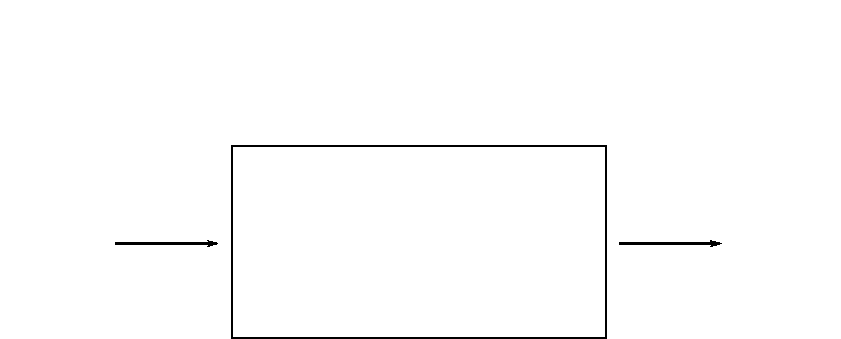
\includegraphics[width=\unitlength,page=1]{pr_model_fig.pdf}}%
    \put(-0.00153098,0.10568847){\color[rgb]{0,0,0}\makebox(0,0)[lb]{\smash{$\rvtup[1],\cdots,\rvtup[n]$}}}%
    \put(0.87700204,0.09818651){\color[rgb]{0,0,0}\makebox(0,0)[lb]{\smash{$\rvhtup[1],\cdots,\rvhtup[n]$}}}%
    \put(0.3225,0.10568842){\color[rgb]{0,0,0}\makebox(0,0)[lb]{\smash{$\Pr\!\left(\rvtup[1],\cdots,\rvtup[n],\rvhtup[1],\cdots,\rvhtup[n]\right)$}}}%
    \put(0,0){\includegraphics[width=\unitlength,page=2]{pr_model_fig.pdf}}%
    \put(0.67828461,0.38248572){\color[rgb]{0,0,0}\makebox(0,0)[lb]{\smash{observable}}}%
  \end{picture}%
\endgroup%

    \caption{The probability model, where a sequence of \emph{plaintext} random queries is transformed into a sequence of random hidden queries.}
    \label{fig:prob_model}
\end{figure}


\subsection{Generative model}
\label{subsec:gen_model}
Consider the time series
\begin{equation}
    \rvtup[1],\ldots,\rvtup[n],\rvhtup[1],\ldots,\rvhtup[n]\,.
\end{equation}
The conditional probability that $\rvtup[n] = \tup[n]$ and $\rvhtup[n] = \htup[n]$ given $\rvtup[<n] = \tup[<n]$ and $\rvhtup[<n] = \htup[<n]$ is given by
\begin{equation}
    \Pr\big[
        \rvhtup[n] = \htup[n], \rvhtup[n] = \htup[n] \given
        \rvtup[<n] = \tup[<n], \rvhtup[<n] = \htup[<n]\big]\,,
\end{equation}
which is equivalent to
\begin{equation}
    \Pr\big[
        \rvts[n] = \ts[n],
        \rvsa[n] = \sa[n],
        \rvqb[n] = \qb[n],    
        \rvhts[n] = \hts[n],
        \rvhsa[n] = \hsa[n],
        \rvhqb[n] = \hqb[n],
        \rvhrs[n] = \hrs[n]
        \given
            \rvhtup[<n] = \htup[<n]\big]\,.
\end{equation}
By the chain rule, this can be rewritten as
\begin{equation}
\begin{split}
    \Pr\big[
        \rvhts[n] = t_n, \rvhsa[n] = a_n, \rvhqb[n] = \hqb[n] &\given \rvhqb[<n] = \hqb[<n]
    \big] =\\
    \Pr\big[
        \rvhts[n] = t_n &\given \rvhqb[<n] = \hqb[<n]
    \big] \times\\
    \Pr\big[
        \rvhsa[n] = a_n &\given \rvhts[n] = t_n, \rvhqb[<n] = \hqb[<n]
    \big] \times\\    
    \Pr\big[
        \rvhqb[n] = \hqb[n] &\given \rvhts[n] = t_n, \rvhsa[n] = a_n, \rvhqb[<n] = \hqb[<n]
    \big]\,.
\end{split}
\end{equation}
The \emph{plaintext} time series of queries \emph{induces} the hidden query time series. If a \emph{simple substitution cipher} is used for the queries and agent identifers and the time stamps are unchanged, then the distribution of hidden queries is the same as the plaintext time series except with different labels.

%Some estimators of $\rv{T_j}$ may be given by a time series estimator like \emph{exponential smoothing}, although this would ignore correlations with other random variables, like $\rv{A_j}$. Regardless, the difficulty with estimating the joint distribution is why we instead focus on the entropy, which has crude estimators in the form of \emph{lossless} compressors.

\begin{algorithm}[h]
    \caption{Generative model of a hidden query time series}
    \label{alg:gen_model}
    \SetKwProg{func}{function}{}{}
    \parameters
    {
        
    }
    \KwIn
    {
        
    }
    \KwOut
    {
        A time series of size $n$ drawn randomly from the induced distribution.
    }
    \func{sampler{$n$}}
    {
        \For{$i \gets 1$ \KwTo $n$}
        {
            sample $\ts[i]$ from $\rvts[i] \given \rvtup[<i] = \tup[<i]$\;
            sample $\sa[i]$ from $\rvsa[i] \given \rvts[i] = \ts[i], \rvtup[<i] = \tup[<i]$\;
            sample $\qb[i]$ from $\rvqb[i] \given \rvsa[i] = \sa[i], \rvts[i] = \ts[i], \rvtup[<i] = \tup[<i]$\;
            $\hsa[i] \gets$ some anonymizer, like a mixnet\;
            $\hts[i] \gets$ something that delays sending hidden query up to some limit\;
            $\hqb[i] \gets \HiddenQueryGenerator(\qb[i] \given \textrm{parameters})$\;
            $\hrs[i] \gets \HiddenQueryMapper(\hqb[i] \given \textrm{parameters})$\;
        }
    }
\end{algorithm}
% RESTRUCTURED: Merged Sections 5-7 (2026-03-22)
% Previously Sections 5 ("Entropy and information"), 6 ("Maximum entropy system"),
% and 7 ("Maximum Entropy Under Constraints") derived maximum-entropy results three
% times with increasing correctness. Section 7 was the cleanest. No content from
% Sections 8+ referenced labels in Sections 5 or 6. The restructured version:
%   - Defines entropy fundamentals once (this section)
%   - Derives max-entropy results once (next section, formerly Section 7)
%   - Relocates performance measure e = H/H* and estimators to end of max-entropy section

\section{Entropy fundamentals}
\label{sec:entropy_fundamentals}
The greater the entropy of the hidden query stream, the fewer patterns an adversary can exploit. In what follows, we define the entropy quantities used throughout the paper.

\begin{definition}[Entropy]
The entropy of the \jth random tuple $\rvhtup[j]$ is given by
\begin{equation}
\label{eq:entropy}
    \entropy\!\left(\rvhtup[j]\right) =
        \mathlarger{\expectation}
        \left[
            \log_2 \pmf_{\mathsmaller{\rvhtup[j]}}\!\left(\rvhtup[j]\right)
        \right]\,,
\end{equation}
where $\pmf_{\mathsmaller{\rvhtup[j]}}\!\left(\,\cdot\,\right)$ is the marginal distribution of $\rvhtup[j]$.
\end{definition}

\begin{definition}[Conditional entropy]
The conditional entropy of the \jth random tuple $\rvhtup[j]$ given the previous $j-1$ random tuples $\rvhtup[<j] \equiv \rvhtup[1],\ldots,\rvhtup[j-1]$ is given by
\begin{equation}
\label{eq:condentropy}
    \entropy\!\left(\rvhtup[j] \given \rvhtup[<j]\right) =
        \mathlarger{\expectation}
        \left[
            \log_2 \pmf_{\mathsmaller{\rvhtup[j] \given \rvhtup[<j]}}
            \left(\rvhtup[j] \given \rvhtup[<j]\right)
        \right]\,.
\end{equation}
\end{definition}

\begin{definition}[Joint entropy]
The joint entropy of $\rvhtup[1], \ldots, \rvhtup[n]$ is given by
\begin{equation}
\label{eq:jointentropy}
    \entropy(\rvhtup[1], \ldots, \rvhtup[n]) =
        \entropy\left(\rvhtup[1]\right) +
        \sum_{j=2}^{n} \entropy\left(\rvhtup[j] \given \rvhtup[<j]\right)\,.
\end{equation}
\end{definition}

The joint entropy is less than (or equal to) the sum of the marginal entropies as given by
\begin{equation}
    \entropy\!\left(\rvhtup[1], \ldots, \rvhtup[n]\right) \leq \sum_{j=1}^{n} \entropy\!\left(\rvhtup[j]\right)\,,
\end{equation}
with equality if and only if $\rvhtup[1], \ldots, \rvhtup[n]$ are statistically independent. If they are independent and identically distributed, then
\begin{equation}
    \entropy\!\left(\rvhtup[1], \ldots, \rvhtup[n]\right) = n \entropy\!\left(\rv{\vec{Q}}\right)\,.
\end{equation}

\begin{postulate}[Optimal compressor]
\label{post:optcomp}
The \emph{entropy} $\entropy\!\left(\rvhtup[1], \ldots, \rvhtup[n]\right)$ is equivalent to the \emph{expected} bit length produced by an optimal \emph{lossless} compressor's output given the encoding of the random tuples as given by
\begin{equation}
    \entropy\left(\rvhtup[1],\ldots,\rvhtup[n]\right) =
    \expectation\Biggl[
        \BL\biggl(
            \Compress^*\bigl(
                \Encode(\rvhtup[1]) \concatop \cdots \concatop \Encode(\rvhtup[n])
                )
            \bigr)
        \biggr)
    \Biggr]\,,
\end{equation}
where $\concatop$ is the concatenation operation, $\Encode$ is an arbitrary encoding of tuples, $\Compress^*$ is an optimal compressor of the sequence, and $\BL(x)$ is the bit length of $x$.
\end{postulate}
The particular codes chosen by the encoder are irrelevant with respect to the entropy of the streams.\footnote{An \emph{optimal} coder is informative about the underlying distribution and thus efficient codes are not necessarily even sought in the context of encrypted search.}

\begin{remark}[Geometric quantization]
The continuous exponential distribution with arrival rate $\lambda$ may be quantized with precision $\tau$ to obtain a geometric distribution with parameter $p = \lambda \tau$. As $\tau \to 0$, the geometric distribution converges to the exponential. The entropy of the quantized (geometric) distribution is
\begin{equation}
    \entropy(\rv{N(\tau)}) = \frac{-(1-p)\log_2(1-p)- p\log_2 p}{p}\,,
\end{equation}
% FIXED: theorem statement now matches the geometric entropy formula in the proof body.
% Previously had an incorrect expansion; counterexample: p=0.25 gave 12.76 vs correct 3.25.
which asymptotically obtains
\begin{equation}
    \lim_{\lambda \tau \to 0} \entropy(\rv{N(\tau)}) = \log_2 \frac{1}{\lambda} + \log_2 \frac{1}{\tau} + \log_2 \mathrm{e}\,.
\end{equation}
This connects the continuous differential entropy $1 + \ln(1/\lambda)$ to the discrete entropy used in the maximum entropy derivations of the next section.
\end{remark}

\section{Maximum Entropy Under Constraints}
\label{sec:maxent}

% RESTRUCTURED: Merged Sections 5-7 (2026-03-22)
In this section, we derive the maximum entropy distribution for encrypted search activities subject to realistic system constraints. The maximum entropy principle, formalized by Jaynes\cite{jaynes1957information}, states that subject to precisely stated prior information, the probability distribution that best represents the current state of knowledge is the one with the largest entropy.

\subsection{System Constraints}
An encrypted search system operates under the following constraints, which we formalize as expectations or support restrictions on the probability distributions:

\begin{enumerate}
    \item \textbf{Query arrival rate}: The mean number of queries per unit time is $\lambda$.
    \item \textbf{Number of search agents}: There are $k$ distinct search agents.
    \item \textbf{Query size}: The mean number of trapdoors per hidden query is $\mu$.
    \item \textbf{Trapdoor vocabulary}: There are $m$ possible distinct trapdoors.
    \item \textbf{Document collection}: There are $N$ distinct documents.
    \item \textbf{Result set size}: The mean number of documents returned per query is $\theta$.
\end{enumerate}

These constraints reflect observable or known properties of the system that cannot be hidden without fundamentally changing the system's functionality or violating resource constraints.

\subsection{Maximum Entropy for Inter-Arrival Times}
The inter-arrival time between consecutive queries is constrained by the arrival rate $\lambda$.

\begin{theorem}[Maximum entropy for inter-arrival times]
Subject to the constraint that $\expectation[\rvhts] = 1/\lambda$, the distribution that maximizes entropy is the exponential distribution:
\begin{equation}
    \rvhts \sim \expdist(\lambda)
\end{equation}
with entropy
\begin{equation}
    \entropy^*(\rvhts) = 1 + \ln \frac{1}{\lambda}\,.
\end{equation}
\end{theorem}

\begin{proof}
Among continuous distributions on $\mathbb{R}_{>0}$ with a fixed mean $1/\lambda$, the exponential distribution maximizes differential entropy. This follows from the calculus of variations applied to the entropy functional subject to the mean constraint. The exponential distribution has probability density function
\begin{equation}
    \pdf_{\rvhts}(t) = \lambda e^{-\lambda t}
\end{equation}
and differential entropy
\begin{equation}
    \entropy(\rvhts) = \int_0^{\infty} -\pdf_{\rvhts}(t) \ln \pdf_{\rvhts}(t) \, dt = 1 + \ln \frac{1}{\lambda}\,.
\end{equation}
\end{proof}

\subsection{Maximum Entropy for Search Agent Identities}
The search agent identity for each query is constrained by the total number of agents $k$.

\begin{theorem}[Maximum entropy for search agent identities]
Subject to the constraint that there are $k$ search agents, the distribution that maximizes entropy is the discrete uniform distribution:
\begin{equation}
    \rvhsa \sim \dudist(1, k)
\end{equation}
with entropy
\begin{equation}
    \entropy^*(\rvhsa) = \log_2 k\,.
\end{equation}
\end{theorem}

\begin{proof}
Among discrete distributions on a finite support of size $k$, the uniform distribution maximizes entropy. The uniform distribution has probability mass function
\begin{equation}
    \pmf_{\rvhsa}(a) = \frac{1}{k} \quad \text{for } a \in \{1, 2, \ldots, k\}
\end{equation}
and entropy
\begin{equation}
    \entropy(\rvhsa) = \sum_{a=1}^{k} -\frac{1}{k} \log_2 \frac{1}{k} = \log_2 k\,.
\end{equation}
\end{proof}

\subsection{Maximum Entropy for Hidden Query Cardinality}
The cardinality of a hidden query (number of trapdoors) is constrained by the mean $\mu$ and typically by a maximum value $u$.

\begin{theorem}[Maximum entropy for query cardinality]
Subject to the constraint that $\expectation[\rv{N_{\text{trap}}}] = \mu$ where $\rv{N_{\text{trap}}} \in \{1, 2, \ldots, u\}$, an approximate maximum entropy distribution is the geometric distribution (when $u$ is large):
\begin{equation}
    \rv{N_{\text{trap}}} \sim \geodist(p)
\end{equation}
where $p = 1/\mu$, with entropy
\begin{equation}
    \entropy^*(\rv{N_{\text{trap}}}) = \frac{-(1-p)\log_2(1-p) - p\log_2 p}{p}\,.
\end{equation}
\end{theorem}

\begin{proof}
The geometric distribution maximizes entropy among discrete distributions on positive integers with a given mean. For $p = 1/\mu$, the geometric distribution has mean $\mu$ and probability mass function
\begin{equation}
    \pmf_{\rv{N}}(n) = p(1-p)^{n-1} \quad \text{for } n \geq 1\,.
\end{equation}
When the maximum value $u$ is large relative to $\mu$, the truncation has negligible effect on the entropy.
\end{proof}

\subsection{Maximum Entropy for Trapdoor Selection}
The trapdoors within a hidden query are drawn from a vocabulary of size $m$.

\begin{theorem}[Maximum entropy for trapdoor selection]
Subject to no constraints beyond the vocabulary size $m$, the distribution that maximizes entropy for each trapdoor is the discrete uniform distribution:
\begin{equation}
    \rv{Y_i} \sim \dudist(1, m)
\end{equation}
with entropy per trapdoor
\begin{equation}
    \entropy^*(\rv{Y_i}) = \log_2 m\,.
\end{equation}
\end{theorem}

\begin{proof}
Without additional constraints on the relative frequencies of trapdoors, the uniform distribution over the vocabulary maximizes entropy. This gives entropy $\log_2 m$ per trapdoor selection.
\end{proof}

% FIXED: MC-2: Removed orphaned "Maximum Entropy for Result Sets" subsection.
% Result set entropy is omitted from the joint formulation since result sets are a
% deterministic function of queries ($H(\mathbf{R} \mid \mathbf{Q}) = 0$).

\subsection{Joint Maximum Entropy}
Combining these results, we obtain the maximum entropy for the complete system.

% FIXED: removed independent result set entropy terms from joint formula.
% Result sets are a deterministic function of queries (see Section~\ref{sec:techniques}),
% so H(result | query) = 0 and result set entropy adds no independent contribution.
\begin{theorem}[Joint maximum entropy]
Under the assumption of independence (which maximizes joint entropy), the maximum entropy for $n$ query tuples is:
\begin{equation}
\begin{split}
    \entropy^*_n &= n \bigg[ \entropy^*(\rvhts) + \entropy^*(\rvhsa) + \entropy^*(\rv{N_{\text{trap}}}) \\
    &\quad + \expectation[\rv{N_{\text{trap}}}] \cdot \entropy^*(\rv{Y}) \bigg]\,.
\end{split}
\end{equation}
\end{theorem}

\begin{remark}
Result set entropy does not appear as an independent term because the result set is a deterministic function of the query: $\entropy(\rvhrs \given \rvhqb) = 0$. Consequently, $\entropy(\rvhqb, \rvhrs) = \entropy(\rvhqb)$, and all result set entropy is already accounted for by the query entropy terms above.
\end{remark}

\begin{proof}
Since entropy is additive for independent random variables, and we assume each query tuple is independent and identically distributed:
\begin{equation}
    \entropy(\rvhtup[1], \ldots, \rvhtup[n]) = \sum_{i=1}^n \entropy(\rvhtup[i]) = n \cdot \entropy(\rvhtup)\,.
\end{equation}
Within each tuple, since result sets are a deterministic function of queries
($\entropy(\rvhrs \given \rvhqb) = 0$), the result set term collapses:
\begin{equation}
    \entropy(\rvhtup) = \entropy(\rvhts) + \entropy(\rvhsa) + \entropy(\rvhqb)\,.
\end{equation}
The entropy of the hidden query bag depends on both the cardinality and the trapdoor selections:
\begin{equation}
    \entropy(\rvhqb) = \entropy(\rv{N_{\text{trap}}}) + \expectation[\rv{N_{\text{trap}}}] \cdot \entropy(\rv{Y})\,.
\end{equation}
\end{proof}

\subsection{Minimum Mutual Information}
The minimum mutual information between plaintext queries $\rvtup[1],\ldots,\rvtup[n]$ and hidden queries $\rvhtup[1],\ldots,\rvhtup[n]$ is achieved when the hidden queries realize the maximum entropy distribution.

\begin{corollary}[Minimum mutual information]
The minimum mutual information is:
\begin{equation}
    \info^{\min}(\rvtup[1:n] ; \rvhtup[1:n]) = \entropy(\rvtup[1:n]) + \entropy^*_n - \entropy_{\max}(\rvtup[1:n], \rvhtup[1:n])
\end{equation}
where $\entropy_{\max}$ represents the maximum possible joint entropy. When the system achieves maximum entropy, the mutual information equals the inherent correlation required by system functionality.
\end{corollary}

This provides a lower bound on information leakage determined by the fundamental requirements of the encrypted search system.

\subsection{Performance Measure and Estimation}

\paragraph{Performance measure.} The performance measure of an encrypted search system is given by the following definition.
\begin{definition}
The performance of an encrypted search system with entropy $\entropy_n$ is given by
\begin{equation}
    e(m,k,\lambda,\mu)=\frac{\entropy_n\left(m, k, \lambda, \mu\right)}{\entropy_n^*(m, k, \lambda, \mu)}\,.
\end{equation}
\end{definition}

A system that obtains $e(\,\cdot\,) = 1$ is said to disclose \emph{minimum information}. Conversely, a system which obtains $e(\,\cdot\,) = 0$ (the degenerate distribution) is said to disclose \emph{maximum information}.\footnote{The Shannon information of a system in which $e(\,\cdot\,) = 0$ is $0$, but we are measuring this with respect to an adversary being able to predict what will happen, so by ``disclose maximum information'' we mean to suggest that it is predictable.}

\paragraph{MLE of maximum entropy.}
If the parameters of the maximum entropy $\entropy_n^*$ are not known, they may be estimated.
\begin{theorem}
The maximum likelihood estimator of $\entropy_n^*$ is given by
\begin{equation}
\label{eq:maxentropy_est}
    \hat{\entropy_n^*} = \entropy_n^*\left(\hat{m}, \hat{k}, \hat{\lambda}, \hat{\mu}\right)\,,
\end{equation}
where $\hat{m}$ is the number of unique trapdoors in the sample, $\hat{k} = \max\{a_1,\ldots,a_n\}$,\footnote{The UMVU estimator of $k$ is given by $\bar{k} = \frac{n + 1}{n} \hat{k}$.} the MLE of $\lambda$ is
\begin{equation}
\label{eq:umvu_lambda_geometric}
    \hat{\lambda} = n \left[\sum_{i=1}^{n} t_i\right]^{-1}\,,
\end{equation}
and the MLE of $\mu$ is
\begin{equation}
    \hat{\mu} = \frac{1}{n} \sum_{i=1}^{n} \Dim(\vec{x_i})\,.
\end{equation}
\end{theorem}

\paragraph{Compression-based entropy estimator.}
If the entropy of the system $\entropy_n$ is not known, it may be estimated via compression.
\begin{theorem}
A \emph{positively biased} estimator of the entropy $\entropy_n$ is given by
\begin{equation}
\label{eq:entropy_est}
    \hat{\entropy}_n =
    \BL\!\left(\Compress
        \left(
            \Concat\!
            \left(
                \Encode\!\left(\vec{q_1}\right),\ldots,\Encode\!\left(\vec{q_n}\right)
            \right)
        \right)
    \right)\,,
\end{equation}
where $q_j = \left(t'_j, a'_j, \vec{x'_j}, \vec{d_j}\right)$ is the \ith observed tuple and $\Compress$ is a \emph{near-optimal} lossless compressor.
\end{theorem}
\begin{proof}
By Postulate~\ref{post:optcomp}, an optimal compressor $\Compress^*$ is expected to produce output whose bit length equals $\entropy_n$. A sub-optimal compressor produces output at least as long, yielding a positively biased estimate.
\end{proof}

% FIXED: MC-3: Deleted asymptotic corollary that confused code length mu(m+1) with
% entropy mu*log2(m), and mixed nats/bits. The correct asymptotic expansion follows
% directly from the joint maximum entropy theorem above.

\begin{corollary}
An estimator of the performance measure is given by
\begin{equation}
    \hat{e} = \frac{\hat{\entropy}_n}{\hat{\entropy}_n^*}\,.
\end{equation}
\end{corollary}
\begin{proof}
By the plug-in principle: if $\hat{\theta}$ is the MLE of $\theta$, then $g(\hat{\theta})$ is the MLE of $g(\theta)$.
\end{proof}

A central idea in this paper is that \emph{compression} is equivalent to \emph{probabilistic} data modeling since a good compressor tends to be a good predictor of the data. Thus, we may delegate the data modeling task to good compressors of encrypted search activities. The more noise-like the activities are, the larger the compressed output.
\section{Increasing the \emph{entropy} of the system}
\label{sec:techniques}
Assuming that the confidential collection of documents is immutable, a given hidden query always maps to the same result set. That is to say, given a hidden query, the corresponding random result set is \emph{degenerate}. Consquently, the \emph{entropy} of the joint distribution of hidden queries and result sets is just the entropy of either distribution,
\begin{equation}
    \entropy(\rvhqb[i], \rvhrs[i]) = \entropy(\rvhqb[i]) = \entropy(\rvhrs[i])\,.
\end{equation}
Thus, the only way to increase the entropy of the result sets is to increase the entropy of the hidden queries. We can thus focus on finding ways to increase the entropy of the hidden queries. 

Note that conditional probability distribution of $\entropy(\rvhrs[i] \given \rvhqb[i]$ is \emph{necessarily} degenerate since a particular hidden query must always map to the same result set. However, $\rvhqb[i] \given \rvhrs[i]$ is not degenerate since many hidden queries may map to the same result set.

Generally, the hidden query stream does not obtain an efficiency of $1$. Thus, we propose to \emph{perturb} the stream to increase the entropy. In this section, we cover general strategies for increasing the entropy at some quantifiable cost.\footnote{In general, this is a non-linear optimization problem where we wish to maximize some function of the entropy and other performance measures.}

The general approach is to interrupt any regularities or patterns in the original stream with unpredictable \emph{noise}, which has the effect of increasing the entropy but decreasing some other performance measure, like the bandwidth requirements of encrypted search activities or the space complexity of the secure indexes.

%This can be accomplished by a more sophisticated \HiddenQueryGenerator which injects \emph{noise} into hidden query such that the set of relevant secure indexes is a superset of the noise-free hidden query.

\subsection{Multiple secure indexes per document}
Ideally, every document in the document store will have an equal probability of being referenced in the stream of result sets. However, this is unlikely since some documents are expected to be generally more relevant to the information needs of the search agents.

Similar to homophonic encryption for trapdoors, a document should be given multiple secure index representations (and more representations in the document store) proportional to the reciprocal of its relative frequency in the stream of result sets. However, there are a few problems with this approach:
\begin{enumerate}
    \item The relative frequency is probably not known a priori.
    \item This increases both the space complexity and time complexity of the encrypted search system since more objects must be stored and queried.
\end{enumerate}

For each document, construct multiple secure indexes in which each secure index for the given document will have a different representation because they will use different document identifiers\footnote{An automated method for generating unique document identifiers may be accomplished by encrypting, using an invertible encryption scheme, the plaintext document reference with different salts.} and different salts for their trapdoors.

This will improve query privacy in a way similiar to homophic encryption. However, homophonic encryption more efficiently serves this purpose. The primary advantage to having multiple secure indexes per document is that it enables the same plaintext query to return a set of logically equivalent results. This \emph{obscures} a user's search patterns, e.g., different users with similar search patterns may sample the salts differently to make their search patterns appear dissimilar.

\begin{example}
Let a document $A$ read ``Hello world!''. Let us represent document $A$ with $N=3$ secure indexes, denoted by $A_1$, $A_2$, and $A_3$. Then, in the biword model, $A_i$’s trapdoors may be generated from the set given by
\begin{equation}
    A_i \gets \MakeSecureIndex\left(\left\{\left(\text{hello} + \text{salt}_i\right)\,, \left(\text{world} + \text{salt}_i\right)\,, \left(\text{hello world} + \text{salt}_i\right)\right\} \given \beta \right)\,.
\end{equation}
\end{example}

This method increases the space and time complexities of encrypted search, e.g., the size of the secure index database grows linearly with respect to $N$.
 
\subsection{Artificial secure indexes}
An extension of multiple secure indexes per document is the automatic inclusion of artificial secure indexes. These may be automatically generated from some language model (e.g., trigram language model) such that they are expected to be relevant to an appropriate percentage of queries.

Artificial secure indexes make it more difficult for an adversary to determine which documents retrieved in response to a hidden query are of actual interest while the user who submitted the search can instantly filter out the fake results. For example, the trapdoor of a artificial secure index document identifier tests positively as a member of the \emph{artificial} document class.



\subsection{Homophonic encryption}
We map the \emph{accuracy} of the adversary with respect to a sample size for various efficiencies in the following analysis. The greater the efficiency (or entropy), the less accurate the mapping is expected to be. At one extreme, we have an efficiency of $0$ (minimum entropy) in which $100\%$ of the traffic is successfully mapped after viewing a sample of size $1$ and the other extreme we have an efficiency of $1$ (maximum entropy) where the accuracy is given by pure random chance and is not correlated with sample size.

\pgfplotstableread{data/0_6.64386_0.1_100_100000} \datazero     % s = 0
\pgfplotstableread{data/0.333333_6.55018_0.1_100_100000} \dataa % s = .33
\pgfplotstableread{data/0.666667_6.14818_0.1_100_100000} \datab % s = .67
\pgfplotstableread{data/1_5.31024_0.1_100_100000} \datac        % s = 1
\pgfplotstableread{data/2_2.26533_0.1_100_100000} \datad        % s = 2
\pgfplotstableread{data/4_0.481547_0.1_100_100000} \datae       % s = 4
\pgfplotstableread{data/8_0.0392275_0.1_100_100000} \dataf      % s = 8
\pgfplotstableread{data/16_0.000266781_0.1_100_100000} \datag   % s = 16
\pgfplotstableread{data/32_7.78651e-09_0.1_100_100000} \datah   % s = 32
\pgfplotstableread{data/64_3.46945e-18_0.1_100_100000} \datai   % s = 64
\pgfplotstableread{data/128_3.76158e-37_0.1_100_100000} \dataj  % s = 128
\pgfplotstableread{data/256_2.21086e-75_0.1_100_100000} \datak  % s = 256
\pgfplotstableread{data/512_3.81867e-152_0.1_100_100000} \datak % s = 512
\pgfplotstableread{data/1024_0_0.1_100_100000} \datal           % s = 1024

\begin{figure}
\caption{Accuracy vs sample size where $N=1000$\\
for several different entropies}
\label{fig:acc_vs_samp_size}
\centering
\begin{tikzpicture}
\begin{axis}
[
    legend cell align = right,
    legend pos = outer north east,
    xmode=log,
    log ticks with fixed point,    
    cycle list name = black white,
    only marks,
    %smooth,
    xmin = 1,
    xmax = 100000,
    ylabel = {accuracy $r$},
    xlabel = {sample size $n$}
]
    \addplot table[y = p] from \datazero;
    \addlegendentry{$e(0,N) = 1.00$};
    %\addlegendentry{$\entropy_1^*(0,N) = 6.64$};
    \addplot table[y = p] from \dataa;
    \addlegendentry{$e\!\left(\frac{1}{3},N\right) = 0.99$};
    %\addlegendentry{$\entropy_1\!\left(\frac{1}{3},N\right) = 6.55$};
    \addplot table[y = p] from \datab;
    \addlegendentry{$e\!\left(\frac{2}{3},N\right) = 0.93$};
    %\addlegendentry{$\entropy_1\!\left(\frac{2}{3},N\right) = 6.15$};
    \addplot table[y = p] from \datac;
    \addlegendentry{$e(1,N) = 0.80$};
    %\addlegendentry{$\entropy_1(1,N) = 5.31$};
    \addplot table[y = p] from \datad;
    \addlegendentry{$e(2,N) = 0.34$};
    %\addlegendentry{$\entropy_1(2,N) = 2.27$};
    \addplot table[y = p] from \datae;
    %\addlegendentry{$\entropy_1(4,N) = 0.48$};
    \addlegendentry{$e(4,N) = 0.07$};
    \addplot table[y = p] from \datah;
    \addlegendentry{$e(\infty,N) = 0.00$};
    %\addlegendentry{$\entropy_1(\infty,N) = 0.00$};
\end{axis}
\end{tikzpicture}
\end{figure}

Homophonic encryption may be employed to flatten the distribution of trapdoors by giving each plaintext word one or more trapdoors signatures.
\begin{figure}
\caption{Testing}
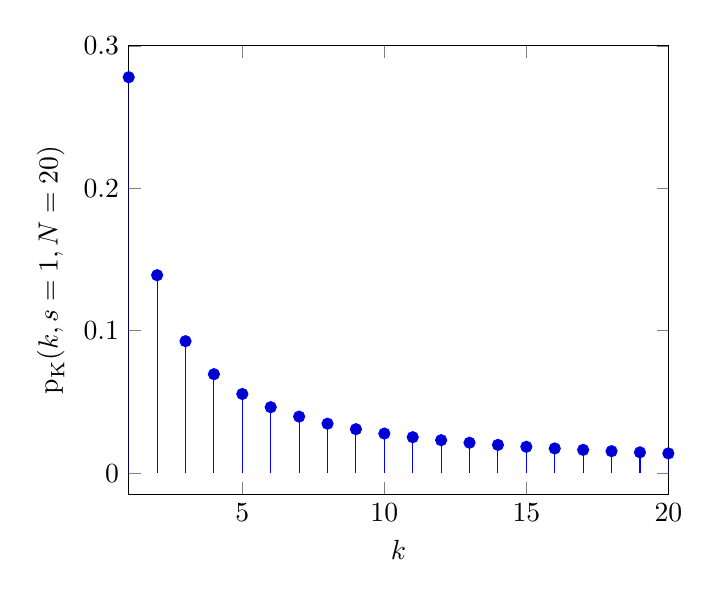
\begin{tikzpicture}
\begin{axis}
[ 
    xlabel=$k$,
    ylabel={$\pmf_{\rv{K}}(k, s=1, N=20)$},
    xmin=1,
    xmax=20,
    ymax=0.3
] 
    \addplot+[ycomb,samples at={1,2,3,4,5,6,7,8,9,10,11,12,13,14,15,16,17,18,19,20}] {1/(x * 3.59774)};
\end{axis}
\end{tikzpicture}
\begin{tikzpicture}
\def\fN(#1,#2){(1/((#1) * 3.59774)/(1/((#2)*3.59774))}
\begin{axis}
[ 
    xlabel=$k$,
    xmin=1,
    xmax=20,
    ymax=0.3
]
    % 1/(1 * 3.59774)*(1/5)     break into 5
    % 1/(2 * 3.59774)*(1/3)     break into 3 (round up from 2.5)
    % 1/(3 * 3.59774)*(1/2)     break into 2 (round up from 1.667)
    % 1/(4 * 3.59774)*(1/1)     break into 2 (round down from 1.25)
    % for a total of 5+3+2+1+(N-4) => N' = N+7 when trying to
    % uniform with respect to the 5th ranked word.
    \addplot+[ycomb,samples at={1,2,3,4}]{1/(x * 3.59774) / round(\fN(x,5))};
    \addplot+[ycomb,samples at={5,6,7,8,9,10,11,12,13,14,15,16,17,18,19,20}] {1/(x * 3.59774)};
\end{axis}
\end{tikzpicture}
\end{figure}

By analyzing queries, a reasonable homophonic code can be devised. However, such trapdoors must be relevant to a corresponding set of secure indexes to facilitate encrypted search. Thus, the more substitutions, the larger the secure indexes. If the space requirements are too demanding to create a completely flat marginal distribution, then we can settle on making the distribution more flat.

%\footnote{Or change the shape of the distribution to counter \emph{known plain-text attacks}}.

Flattening the \emph{marginal} distribution does not prevent adversaries from learning mappings since random plain-text words $\rv{T_j}$ and $\rv{T_k}$ are not necessarily statistically independent and, for instance, may still have a \emph{non-uniform} conditional distribution
\begin{equation}
    \rv{T_j} \given \rv{T_k} \sim \pmf_{\rv{T_j} \given \rv{T_k}}\!\left(\;\cdot\;\right)\,.
\end{equation}





\begin{algorithm}
    \caption{Homophonic substitution cipher}
    \label{alg:homphon_sub}
    \SetKwProg{func}{function}{}{}
    \parameters
    {
        $b$, maximize the \emph{marginal} entropy of the distribution of trapdoors up to the $b$-th ranked word.
    }
    \KwIn
    {
        A \emph{plaintext} word $x$.

    }
    \KwOut
    {
        A trapdoor $\check{x}$ of plaintext word $x$\;
    }
    \func{\substitutions{$x$}}
    {
        \tcp{Retrieve the $b$-th ranked word and compute its \emph{relative frequency}.}
        $\beta \gets \pmf_{\rv{X}}\!\left(\Rank^{-1}(b)\right)$\;
        $m \gets 1$\;
        \tcp{If the rank of $x$ is less than $b$, we must provide
        more than $1$ possible substitution such that the first
        $b$ words are (approximately) uniformly distributed.}
        \If{$\Rank(x) < b$}
        {
            $m \gets \left\lfloor
                \frac
                {
                    \pmf_{\rv{X}}(x)
                }
                {
                    \beta
                } + \frac{1}{2}
            \right\rfloor$\;
        }
        \Return $m$\;
    }
\end{algorithm}

\subsection{Query aggregation}
Instead of submitting a single query consisting of $k$ search keys, we can reduce it to $y$ queries where the \jth query has $k_j$ search keys for $j=1,\ldots,y$ such that $k_1 + \cdots + k_y = k$ and then apply the \emph{set-intersection} operation on the $y$ result sets on a \emph{trusted machine}, such as the search agent's host computer rather than the untrusted encrypted search provider.

\begin{remark}
A query model that includes the full set-theoretic model\cite{manning2008introduction} may reveal significantly more information about a search agent's information need. Thus, if a full set-theoretic model is desired, a strong case can be made that it should be implemented using a variation of query aggregation, where set-theoretic operations (with possibly the exception of set-intersection) are applied to the result sets on a \emph{trusted} machine rather than the \emph{untrusted} encrypted search provider.
\end{remark}

\subsection{\emph{Artificial} trapdoors}
The effectiveness of artificial trapdoors depends critically on the encrypted search provider's ranking mechanism. In boolean search systems where all query terms must be present for document retrieval, artificial trapdoors will cause no matching documents to be returned, making this technique ineffective. However, for rank-ordered retrieval systems using scoring functions such as BM25 or TF-IDF, artificial trapdoors integrate seamlessly with authentic trapdoors. In such systems, artificial trapdoors affect result sets only when: (1) they trigger false positives in secure indexes due to the approximate nature of structures like Bloom filters, or (2) they coincidentally collide with authentic trapdoors due to the finite trapdoor space.

The probability of collision between artificial and authentic trapdoors is governed by the birthday paradox. With $m'$ authentic trapdoors and $m''$ artificial trapdoors drawn uniformly from a space of size $2^l$, the expected number of collisions is approximately $\frac{m' \cdot m''}{2^l}$. For typical systems with $l \geq 128$ bits, collision probability remains negligible even with thousands of artificial trapdoors.

Suppose that each query has some random number $\rv{L}$ of \emph{artificial} trapdoors, where
\begin{equation}
    \rv{L} \sim \pmf_{\rv{L}}(\,\cdot\,\given \mu_{\rv{L}})
\end{equation}
such that
\begin{equation}
    \expectation\!\left[\rv{L}\right] = \mu_{\rv{L}}\,.
\end{equation}
Let the random variable corresponding to the artificial trapdoor be given by
\begin{equation}
    \rv{Y} \sim \pmf_{\rv{Y}}(\,\cdot\,\given m_{\rv{Y}})\,,
\end{equation}
where $m_{\rv{Y}}$ is the number of unique artificial trapdoors.

The maximum entropy of the joint distribution of $\rv{L}$ and $\rv{Y}$ is given by the following theorem.
\begin{theorem}
\begin{equation}
    \entropy^*(\rv{L},\rv{Y}) = \entropy^*(\rv{L} \given \mu_{\rv{L}},\rv{Y})
\end{equation}
\end{theorem}

Suppose we have $l$ bits per trapdoor, then at maximum we may generate $m'' = 2^l - m'$ artificial trapdoors, where $m'$ are the unique number of bit patterns corresponding to \emph{authentic} trapdoors. 

Letting $\rv{M}$ and $\rv{T'_j}$ for all $j$ be independent, then the mean number of \emph{authentic} and \emph{artificial} trapdoors per query is given by
\begin{equation}
    \mu'' = \mu' + \mu'_{\rv{L}}\,.
\end{equation}

If we randomize the order of the trapdoors in the hidden queries and let $\mu'_{\rv{L}} \to \infty$, then the efficiency of the entire encrypted search system will converge to
\begin{equation}
    e(\mu'') = \frac
    {
        \entropy_n(\rv{N},\rv{\vec{Y}} \given \mu'')
    }
    {
        n \entropy^*(\rv{N},\rv{\vec{Y}} \given \mu'')
    }\,.
\end{equation}

Assume the adversary has a model of the hidden query stream using known-plaintext attacks. Perturbing the hidden query stream by adding \emph{noise} to it may counter known-plaintext attacks. Alternatively, assume that the adversary knows the secret and thus may use a dictionary attack to decipher the trapdoors. Then, adding noise may in some cases obfuscate what a search agent is actually interested in. 

To mitigate such information leaks, in general we can look to oblivious RAM for inspiration. oblivious RAM may naively be thought of in the following way: to prevent meaningful statistics from being gathered about a user’s activities, whenever an action--a read or write--is performed, include other randomly chosen actions to obscure the user’s actual interests or activities.

\subsection{\emph{Artificial} hidden queries}
%\begin{figure}
%\caption{\emph{Faux} hidden query injector.}
%\label{fig:fake_q_inject}
%\center
%\def\svgwidth{\textwidth}
%%% Creator: Inkscape inkscape 0.92.1, www.inkscape.org
%% PDF/EPS/PS + LaTeX output extension by Johan Engelen, 2010
%% Accompanies image file 'perturbed_fake_query.pdf' (pdf, eps, ps)
%%
%% To include the image in your LaTeX document, write
%%   \input{<filename>.pdf_tex}
%%  instead of
%%   \includegraphics{<filename>.pdf}
%% To scale the image, write
%%   \def\svgwidth{<desired width>}
%%   \input{<filename>.pdf_tex}
%%  instead of
%%   \includegraphics[width=<desired width>]{<filename>.pdf}
%%
%% Images with a different path to the parent latex file can
%% be accessed with the `import' package (which may need to be
%% installed) using
%%   \usepackage{import}
%% in the preamble, and then including the image with
%%   \import{<path to file>}{<filename>.pdf_tex}
%% Alternatively, one can specify
%%   \graphicspath{{<path to file>/}}
%% 
%% For more information, please see info/svg-inkscape on CTAN:
%%   http://tug.ctan.org/tex-archive/info/svg-inkscape
%%
\begingroup%
  \makeatletter%
  \providecommand\color[2][]{%
    \errmessage{(Inkscape) Color is used for the text in Inkscape, but the package 'color.sty' is not loaded}%
    \renewcommand\color[2][]{}%
  }%
  \providecommand\transparent[1]{%
    \errmessage{(Inkscape) Transparency is used (non-zero) for the text in Inkscape, but the package 'transparent.sty' is not loaded}%
    \renewcommand\transparent[1]{}%
  }%
  \providecommand\rotatebox[2]{#2}%
  \ifx\svgwidth\undefined%
    \setlength{\unitlength}{540.3682838bp}%
    \ifx\svgscale\undefined%
      \relax%
    \else%
      \setlength{\unitlength}{\unitlength * \real{\svgscale}}%
    \fi%
  \else%
    \setlength{\unitlength}{\svgwidth}%
  \fi%
  \global\let\svgwidth\undefined%
  \global\let\svgscale\undefined%
  \makeatother%
  \begin{picture}(1,0.39245497)%
    \put(0,0){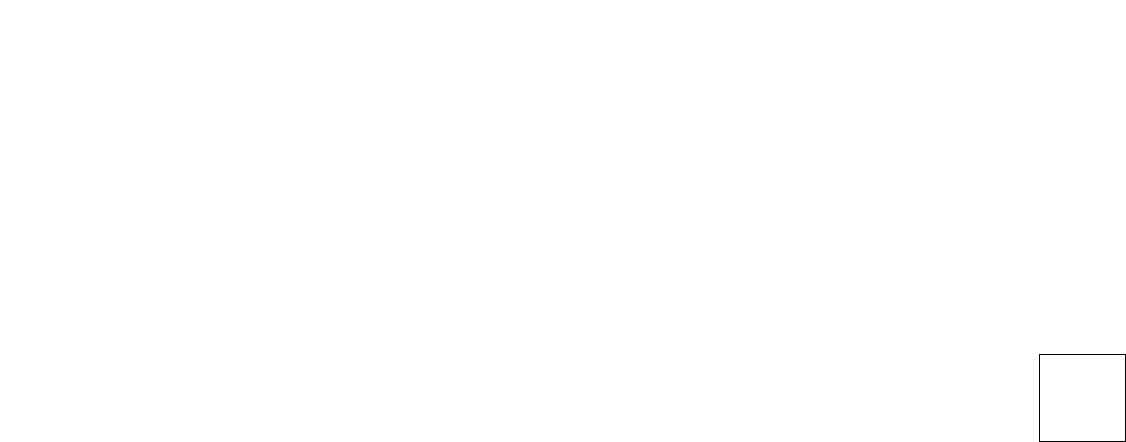
\includegraphics[width=\unitlength,page=1]{perturbed_fake_query.pdf}}%
    \put(0.94121535,0.03158698){\color[rgb]{0,0,0}\makebox(0,0)[lb]{\smash{ESP}}}%
    \put(0.38071106,0.01107937){\color[rgb]{0,0,0}\makebox(0,0)[lb]{\smash{\emph{perturbed} HQ stream}}}%
    \put(0,0){\includegraphics[width=\unitlength,page=2]{perturbed_fake_query.pdf}}%
    \put(0.01175919,0.03158703){\color[rgb]{0,0,0}\makebox(0,0)[lb]{\smash{Obfuscator}}}%
    \put(3.33764174,-2.20660118){\color[rgb]{0,0,0}\makebox(0,0)[lt]{\begin{minipage}{0.57622423\unitlength}\raggedright \end{minipage}}}%
    \put(0,0){\includegraphics[width=\unitlength,page=3]{perturbed_fake_query.pdf}}%
    \put(-0.02238722,-0.0642656){\color[rgb]{0,0,0}\makebox(0,0)[lb]{\smash{}}}%
    \put(-0.01941306,-0.05038613){\color[rgb]{0,0,0}\makebox(0,0)[lb]{\smash{}}}%
    \put(0.5179189,0.07948564){\color[rgb]{0,0,0}\makebox(0,0)[lt]{\begin{minipage}{0.25875208\unitlength}\raggedright \end{minipage}}}%
    \put(0.2,0.0625){\color[rgb]{0,0,0}\makebox(0,0)[lb]{\smash{$\left(t_1,a_{j_1},\vec{y'_1}\right),\left(t_2,a_{j_2},\vec{y_2}\right),\left(t_3,a_{j_3},\vec{y'_3}\right),\left(t_4,a_{j_4},\vec{y_4}\right),\left(t_5,a_{j_5},\vec{y'_5}\right),\,\cdots$}}}%
    \put(0.21158019,0.05470089){\color[rgb]{0,0,0}\makebox(0,0)[lb]{\smash{}}}%
    \put(0,0){\includegraphics[width=\unitlength,page=4]{perturbed_fake_query.pdf}}%
    \put(0.37317635,0.35013436){\color[rgb]{0,0,0}\makebox(0,0)[lb]{\smash{\emph{Faux} HQ injector}}}%
    \put(0,0){\includegraphics[width=\unitlength,page=5]{perturbed_fake_query.pdf}}%
  \end{picture}%
\endgroup%

%\end{figure}
Unlike artificial trapdoors which may alter result sets through collisions or false positives, artificial queries are designed to be distinguishable by the search agent while appearing indistinguishable to the adversary. The search agent can filter out artificial queries from result sets using cryptographic tags or sequence numbers, ensuring that authentic queries receive unmodified results. This approach trades space complexity for time and bandwidth: instead of expanding the trapdoor space through homophonic encryption (Section~\ref{subsec:homophonic}), we expand the temporal query stream.

The choice of query representation (unigrams, bigrams, trigrams, or longer n-grams) significantly impacts the entropy-confidentiality tradeoff. Unigram queries provide a vocabulary of size $|V|$, yielding at most $\log_2 |V|$ bits of entropy per trapdoor. Bigram queries expand the space to $|V|^2$ possibilities, increasing per-trapdoor entropy to $2\log_2 |V|$ bits at the cost of larger secure indexes. Position-sensitive representations like skip-grams or phrase queries further expand the trapdoor space while supporting richer search semantics.

To increase the entropy of the hidden queries without the space complexity costs associated with homophonic encryption (see Section~\ref{subsec:homophonic}) but rather with a \emph{time complexity} and \emph{transmission rate} cost, we may inject \emph{artificial} queries into the hidden query stream.

To increase the entropy, the \emph{artificial} queries should be injected into the stream to make the hidden query stream less correlated.
\begin{example}
Consider the \emph{authentic} hidden query stream given by
\begin{equation}
    (t_1, a_{j_1}, \vec{y_1}), (t_2, a_{j_1}, \vec{y_2}), (t_3, a_{j_1}, \vec{y_3})\,.
\end{equation}
There may be patterns in this sequence, such as autocorrelations between $\vec{y_1}$, $\vec{y_2}$, and $\vec{y_3}$. If we inject the \emph{artificial} queries $\vec{y'_1}$ and $\vec{y'_2}$ into the stream, resulting in the \emph{perturbed} hidden query stream given by
\begin{equation}
    (t_1, a_{j_1}, \vec{y_1}), (t'_1, \cdot, \vec{y'_1}), (t_2, a_{j_2}, \vec{y_2}), (t'_2, \cdot, \vec{y'_2}), (t_3, a_{j_3}, \vec{y_3})\,,
\end{equation}
where $t_1 \leq t'_1 \leq t_2 \leq t'_2 \leq t_3$. The \emph{perturbed} stream may attenuate\footnote{And therefore increases the entropy.} any regularities such as auto-correlations.
\end{example}

The entropy of this \emph{perturbed} stream is maximally increased when the time stamps are geometrically distributed with a mean query rate $\check{\lambda}$ per search agent, the search agent identities are uniformly distributed between $1$ and $\check{k}$, the cardinality of the trapdoor sets are binomially distributed between $1$ and $\check{m}$ with a mean $\check{\mu}$, and the trapdoors are uniformly distributed between $1$ and $\check{m}$.

This technique does not transform \emph{authentic} hidden queries. However, as $\check{\lambda}$ increases due to injecting \emph{artificial} hidden queries, patterns become attenuated. Asymptotically, as $\check{\lambda} \to \infty$, the distribution of hidden query converges to the maximum entropy distribution. Of course, asymptotically, infinite bandwidth and computational resources are required.

\subsubsection{Alternative solution}
A potential problem with previous solution of increasing the entropy is that the obfuscator must inject \emph{artificial} hidden queries without prompting from the search agent. If this is impractical, then a less effective solution -- one that only increases the entropy of the trapdoors -- is for search agents to (automatically) generate random \emph{artificial} hidden queries whenever they generate \emph{authentic} hidden queries.

To maximize the entropy under these constraints, the \emph{artificial} hidden queries are generated in the following ways:
\begin{enumerate}
\item The time stamps of the queries are randomized to change the order of the query submissions.\footnote{The time stamps are approximately the same.} Thus, if $r$ hidden queries are generated, there are $r!$ possible orderings each of which is equally probable.
\item The random cardinality of each trapdoor set in the \emph{artificial} hidden queries is binomially distributed with a mean $\check{\theta}$ with a maximum value of $\check{m}$.
\item Each element of the trapdoor set is uniformly distributed with a support set $\{1,\ldots,\check{m}\}$.
\item The random number of \emph{artificial} queries is geometrically distributed with a mean rate given by $\check{\lambda}$ with a support set $\{0,1,2,\ldots\}$ and thus each \emph{authentic} hidden query has on average $\frac{1-\check{\lambda}}{\check{\lambda}}$ \emph{artificial} hidden queries bundled with it.
\end{enumerate}

\subsection{Obfuscating search agents}
%Returning a mapping from hidden query to result set to a particular search agent requires that the search agent be identified in some way, e.g., an IP address. In the encrypted search model, a particular query interaction is denoted by the tuple $(t, a, \vec{y}, \vec{d})$, where $a$ is the search agent identifier.

The adversary may observe the time series of hidden queries. By analyzing the network traffic going to and from the ESP, the adversary may be able to uniquely label the search agents generating the hidden queries, especially if no precautionary measures are taken to obfuscate this identifying\footnote{For instance, IP addresses.} information.

A mix network\cite{chaum1981untraceable} is an overlay network that may obscure the identities of search agents.

An \emph{onion network} is another type of overlay network...

The \emph{maximum uncertainty} occurs when there is no identifying information. Consequently, given that the adversary knows there are $k$ unique search agents, the probability that a particular search agent is responsible for a particular hidden query is $1 / k$ with an entropy given by $\log_2 k$.

A mix network helps, but search agents may have identifying search patterns, i.e., search agent $j$ may be more likely to generate queries in particular intervals of time. These correlations may be obfuscated using other methods discussed previously.

\subsection{Injecting \emph{artificial} search agents}
To increase the entropy, \emph{artificial} search agents may be introduced that generate \emph{artificial} hidden queries. If there are $k$ authentic search agents and $w$ artificial search agents, then there are $k' = k + w$ search agents in total.

If $k$ is known, then the maximum entropy distribution is the same as before, the discrete uniform distribution over $k$ search agents with an entropy given by $\entropy(\rvhsa \given k) = \log_2 k$. Of course, in practice the maximum entropy may not be achieved and introducing artificial search agents may increase the entropy.

However, if $k$ is not known, but $k'$ is, then $k$ may be modeled as a random variable $\rv{K}$ with a support given by $\{0,1,\ldots,k'\}$.

The joint distribution of $(\rvhsa, \rv{K})$ has an entropy given by
\begin{equation}
    \entropy(\rvhsa, \rv{K}) = \entropy(\rvhsa \given \rv{K}) + \entropy(\rv{K})
\end{equation}
with a maximum entropy given by
\begin{equation}
    \entropy(\rvhsa \given \rv{K}) + \entropy(\rv{K})\,.
\end{equation}
\begin{equation}
    \entropy(\rvhsa \given \rv{K}) + \log_2 k' + \log_2 k'\,.
\end{equation}
If $\pmf_{\rv{K}}(k \given k')$ is degenerate and assigns all the probability to the authentic number of search agents, then the entropy...

\subsection{Obfuscating inter-arrival times}
If the query arrival rate is $\lambda$, then the maximum entropy distribution of inter-arrival times in the hidden query time series is exponentially distributed with a rate $\lambda$, denoted by
\begin{equation}
    \rvhts \sim \expdist(\lambda)\,.
\end{equation}
%As a side-note, this means that the queries are a Poisson process.

We use queuing theory to characterize the query arrival times where we consider the \emph{obfuscator} to be the server and the \emph{search agents} to be the customers.

The arrival times are the times that plaintext queries are received by the obfuscator; when a query arrives, it is put into the queue and the obfuscator ``serves'' queries at the \emph{head} of the queue.

If over an interval of time $\Delta t$ the obfuscator receives $n$ queries, then the average inter-arrival time over that interval of time is simply $\Delta t / n$ and the arrival rate is $\lambda = n / \Delta t$. More specifically, suppose we have $n$ plaintext queries with inter-arrival times $\ts[1],\ldots,\ts[n]$. The \emph{mean} inter-arrival time is
\begin{equation}
    \bar{t} = \frac{1}{n} \sum_{j=1}^{n} \ts[j]\,,
\end{equation}
and therefore the arrival rate is
\begin{equation}
    \lambda = \frac{1}{\bar{t}}\,.
\end{equation}
We assume $\ts[j]$ follows a probability distribution $\rvts[j]$ for $j=1,\ldots,n$. To \emph{reshape} the arrival times at the ESP, the obfuscator may \emph{delay} sending hidden queries to the ESP. Under the queuing theory model, the delay may be considered the \emph{service time}. If the \emph{mean} service time is $\mu$, then the \emph{service rate} is $1 / \mu$. To keep up with the query arrival rate, the service rate must be $\lambda$, i.e., $\mu = 1 / \lambda$, which is equivalent to the mean inter-arrival time.

\begin{theorem}
Suppose we have $k$ search agents with query rates $\lambda_1, \ldots, \lambda_k$. If each uses an obfuscator to transform the inter-arrival times to be exponentially distributed with arrival rates $\lambda_1, \ldots, \lambda_k$, then the collective inter-arrival times is exponentially distributed with an arrival rate $\lambda_1 + \cdots + \lambda_k$.
\end{theorem}
\begin{proof}
The sum of $k$ independent Poisson processes with rates $\lambda_1, \ldots, \lambda_k$ is itself a Poisson process with rate $\lambda = \sum_{j=1}^{k} \lambda_j$. This is a standard result in stochastic processes.

To verify, let $N_i(t)$ denote the counting process for agent $i$, where $N_i(t) \sim \poissondist(\lambda_i t)$. The superposition $N(t) = \sum_{i=1}^{k} N_i(t)$ counts arrivals from all agents. By independence and the additive property of Poisson random variables,
\begin{equation}
    N(t) \sim \poissondist\left(\sum_{i=1}^{k} \lambda_i t\right) = \poissondist(\lambda t)\,.
\end{equation}
Since a Poisson process has exponentially distributed inter-arrival times, the collective inter-arrival times follow $\expdist(\lambda)$.
\end{proof}


\begin{figure}
\caption{Inter-arrival time obfuscation}
\label{fig:inter_arrival_perturb}
\center
\def\svgwidth{\textwidth/2}
%% Creator: Inkscape inkscape 0.92.1, www.inkscape.org
%% PDF/EPS/PS + LaTeX output extension by Johan Engelen, 2010
%% Accompanies image file 'inout.pdf' (pdf, eps, ps)
%%
%% To include the image in your LaTeX document, write
%%   \input{<filename>.pdf_tex}
%%  instead of
%%   \includegraphics{<filename>.pdf}
%% To scale the image, write
%%   \def\svgwidth{<desired width>}
%%   \input{<filename>.pdf_tex}
%%  instead of
%%   \includegraphics[width=<desired width>]{<filename>.pdf}
%%
%% Images with a different path to the parent latex file can
%% be accessed with the `import' package (which may need to be
%% installed) using
%%   \usepackage{import}
%% in the preamble, and then including the image with
%%   \import{<path to file>}{<filename>.pdf_tex}
%% Alternatively, one can specify
%%   \graphicspath{{<path to file>/}}
%% 
%% For more information, please see info/svg-inkscape on CTAN:
%%   http://tug.ctan.org/tex-archive/info/svg-inkscape
%%
\begingroup%
  \makeatletter%
  \providecommand\color[2][]{%
    \errmessage{(Inkscape) Color is used for the text in Inkscape, but the package 'color.sty' is not loaded}%
    \renewcommand\color[2][]{}%
  }%
  \providecommand\transparent[1]{%
    \errmessage{(Inkscape) Transparency is used (non-zero) for the text in Inkscape, but the package 'transparent.sty' is not loaded}%
    \renewcommand\transparent[1]{}%
  }%
  \providecommand\rotatebox[2]{#2}%
  \ifx\svgwidth\undefined%
    \setlength{\unitlength}{429.98562493bp}%
    \ifx\svgscale\undefined%
      \relax%
    \else%
      \setlength{\unitlength}{\unitlength * \real{\svgscale}}%
    \fi%
  \else%
    \setlength{\unitlength}{\svgwidth}%
  \fi%
  \global\let\svgwidth\undefined%
  \global\let\svgscale\undefined%
  \makeatother%
  \begin{picture}(1,0.91389413)%
    \put(0,0){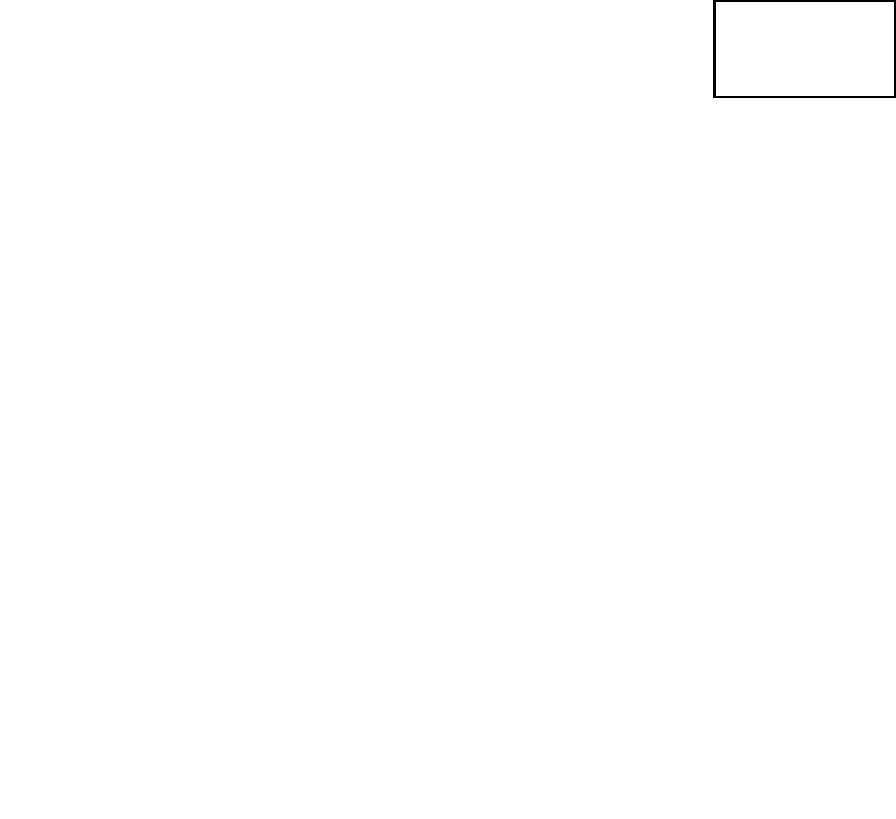
\includegraphics[width=\unitlength,page=1]{inout.pdf}}%
    \put(0.81,0.85){\color[rgb]{0,0,0}\makebox(0,0)[lb]{\smash{\footnotesize{obfuscator}}}}%
    \put(-0.01287918,1.11588507){\color[rgb]{0,0,0}\makebox(0,0)[lt]{\begin{minipage}{0.31663073\unitlength}\raggedright \end{minipage}}}%
    \put(0,0){\includegraphics[width=\unitlength,page=2]{inout.pdf}}%
    \put(0.025,0.845){\color[rgb]{0,0,0}\makebox(0,0)[lb]{\smash{SA}}}%
    \put(0.01702215,1.03365639){\color[rgb]{0,0,0}\makebox(0,0)[lt]{\begin{minipage}{0.86713864\unitlength}\raggedright \end{minipage}}}%
    \put(-0.13497628,1.42984905){\color[rgb]{0,0,0}\makebox(0,0)[lt]{\begin{minipage}{0.91946603\unitlength}\raggedright \end{minipage}}}%
    \put(0,0){\includegraphics[width=\unitlength,page=3]{inout.pdf}}%
    \put(0.18821872,0.826){\color[rgb]{0,0,0}\makebox(0,0)[lb]{\smash{\Large{*}}}}%
    \put(0.64190657,0.826){\color[rgb]{0,0,0}\makebox(0,0)[lb]{\smash{\Large{*}}}}%
    \put(0.29305761,0.826){\color[rgb]{0,0,0}\makebox(0,0)[lb]{\smash{\Large{*}}}}%
    \put(0,0){\includegraphics[width=\unitlength,page=4]{inout.pdf}}%
    \put(0.45370615,0.683){\color[rgb]{0,0,0}\makebox(0,0)[lb]{\smash{$\ts[2]$}}}%
    \put(0.24377396,0.683){\color[rgb]{0,0,0}\makebox(0,0)[lb]{\smash{$\ts[1]$}}}%
    \put(0,0){\includegraphics[width=\unitlength,page=5]{inout.pdf}}%
    \put(0.8676,0.69488612){\color[rgb]{0,0,0}\rotatebox{-90}{\makebox(0,0)[lb]{\smash{\Large{*}}}}}%
    \put(0.8676,0.26562168){\color[rgb]{0,0,0}\rotatebox{-90}{\makebox(0,0)[lb]{\smash{\Large{*}}}}}%
    \put(0.8676,0.48888206){\color[rgb]{0,0,0}\rotatebox{-90}{\makebox(0,0)[lb]{\smash{\Large{*}}}}}%
    \put(0,0){\includegraphics[width=\unitlength,page=6]{inout.pdf}}%
    \put(0.727,0.365){\color[rgb]{0,0,0}{\makebox(0,0)[lb]{\smash{$\hts[2]$}}}}%
    \put(0.727,0.575){\color[rgb]{0,0,0}{\makebox(0,0)[lb]{\smash{$\hts[1]$}}}}%
    \put(0,0){\includegraphics[width=\unitlength,page=7]{inout.pdf}}%
    \put(0.855,0.04){\color[rgb]{0,0,0}\makebox(0,0)[lb]{\smash{ESP}}}%
  \end{picture}%
\endgroup%

\end{figure}



\begin{remark}
Intuitively, the \emph{no-memory property} of the exponential distribution is indicative of its maximum entropy. However, if we allow the support to be constrained over $0$ to $2 / \lambda$, then the uniform distribution obtains the same entropy $\ln \lambda$ such that $\expectation[\rvhts] = 1 / \lambda$. 
\end{remark}


\subsubsection{Estimating search agent arrival rates}
The $k$ search agents have query arrival rates $\lambda_1, \cdots, \lambda_k$ which may be unknown to the adversary. Assuming the obfuscators transform the inter-arrival times to be exponentially distributed, the queries collectively arrive with inter-arrival times distributed exponentially with an arrival rate $\lambda = \lambda_1 + \cdots + \lambda_k$, which may be observed by the adversary.

Estimating the arrival rates of the search agents may be revealing. Suppose that the adversary, by some process, has a sample of inter-arrival times (and corresponding hidden queries and result sets) along with a set of \emph{candidate} search agents who were the most likely to have submitted the query (or, alternatively, it is known that one of the candidates submitted the query).

Then, the arrival rates may be estimated from this sample of the \emph{masked} search agents.

To describe the output process of the queuing system, the probability distribution for the service time distribution which governs a ``customer’s'' service time. We assume the service time distribution is independent of the number of customers present. This implies, for example, that the server does not work faster when more customers are present.

The obfsucator could impose a service delay that is exactly the inter-arrival time $1 / \lambda_j$ rather than creating a traffic flow that is exponentially distributed with a mean inter-arrival time $1 / \lambda_j$. In this case, the adversary can only guess that the average number of queries per day is $24 \lambda$ queries per day. However, if the queries are not uniformly distributed, it is not be possible (without introducing \emph{fake} queries) to maintain this constant delay, which reveals information about the distribution of query times.



Queue discipline:
FCFS discipline - first come first serve
SORS discipline - service in random order


Suppose we have $k$ search agents, where search agent $j$ has a query rate $\lambda_j$. Then, the total query rate is $\lambda = \lambda_1 + \cdots + \lambda_k$.

If the search agents are unable to effectively anonymize their identities, then a strategy for confidentiality is to put the queries into a local queue and have the queue \emph{emit} the queries in such a way that the inter-arrival times are \emph{exponentially} distributed with an arrival rate $\lambda_j$.

Of course, if queries come in bursts as is often the case (that is, the inter-arrival times exhibit large variance), then the queue must \emph{delay} queries.

may cause significant delays. Additionally, if there are no queries in the queue due to the bu



If the encrypted search system is receiving queries at a rate $\lambda$, then on average each of the $k$ search agent is sending queries at a rate $\lambda / k$





\section{Case Study: Typical Encrypted Search System}
\label{sec:casestudy}

In this section, we analyze a typical encrypted search deployment to demonstrate the practical application of our information-theoretic framework. We compare the entropy of actual system behavior against the maximum entropy possible under system constraints, quantifying the confidentiality gap and proposing targeted improvements.

\subsection{System Parameters}
Consider an encrypted search system with the following characteristics, representative of a small organizational deployment:

\begin{table}[h]
    \centering
    \caption{Parameters for case study system}
    \label{tbl:case_study_params}
    \begin{tabular}{@{} l l l @{}}
        \toprule
        \textbf{Parameter} & \textbf{Value} & \textbf{Description}\\
        \midrule
        $k$ & 10 & Number of search agents\\
        $m$ & 10,000 & Distinct words in query vocabulary\\
        $N$ & 1,000 & Documents in collection\\
        $\lambda$ & 0.1 & Query arrival rate (queries per second)\\
        $\mu$ & 3 & Mean trapdoors per query\\
        $u$ & 10 & Maximum trapdoors per query\\
        $\theta$ & 5 & Mean documents per result set\\
        \bottomrule
    \end{tabular}
\end{table}

\subsection{Baseline: Simple Substitution Cipher}
We first analyze a simple substitution cipher where each word maps to a single trapdoor with no additional obfuscation.

\subsubsection{Observed Distribution}
In a typical query workload following a Zipf distribution, the query word frequencies are highly skewed:
\begin{equation}
    \pmf_{\rv{X}}(x_i) \propto \frac{1}{i} \quad \text{for word ranked } i
\end{equation}

This creates a highly non-uniform trapdoor distribution:
\begin{equation}
    \pmf_{\rv{Y}}(y_i) = \pmf_{\rv{X}}(x_i) \propto \frac{1}{i}
\end{equation}

\subsubsection{Entropy Calculation}
The entropy of the trapdoor distribution under Zipf's law with parameter $s=1$ is:
\begin{equation}
    \entropy(\rv{Y}) = \sum_{i=1}^{m} -\frac{1}{i H_{m,1}} \log_2 \frac{1}{i H_{m,1}}
\end{equation}
where $H_{m,1} = \sum_{i=1}^{m} 1/i$ is the $m$-th harmonic number.

For $m=10{,}000$, we have $H_{10000,1} \approx 9.787$, giving:
\begin{equation}
    \entropy(\rv{Y}) \approx 7.83 \text{ bits}
\end{equation}

Compare this to the maximum entropy:
\begin{equation}
    \entropy^*(\rv{Y}) = \log_2 10{,}000 = 13.29 \text{ bits}
\end{equation}

\subsubsection{Efficiency}
The ratio of actual to maximum entropy for trapdoors is:
\begin{equation}
    e_{\text{trap}} = \frac{7.83}{13.29} \approx 0.59
\end{equation}

For complete queries with mean 3 trapdoors:
\begin{equation}
    \entropy(\rvhqb) \approx 3 \times 7.83 = 23.49 \text{ bits}
\end{equation}
versus maximum:
\begin{equation}
    \entropy^*(\rvhqb) \approx 3 \times 13.29 = 39.87 \text{ bits}
\end{equation}

The query efficiency is similarly $e_{\text{query}} \approx 0.59$.

\subsection{Improvement 1: Homophonic Encryption}
\label{subsec:homophonic}
We apply homophonic encryption to flatten the trapdoor distribution, giving the top $b$ most frequent words multiple trapdoor representations.

\subsubsection{Strategy}
For the $b=100$ most frequent words, assign trapdoor multiplicities inversely proportional to their frequency:
\begin{equation}
    n_i = \left\lceil \frac{\pmf_{\rv{X}}(x_1)}{\pmf_{\rv{X}}(x_i)} \right\rceil \quad \text{for } i \leq b
\end{equation}

This approximately flattens the distribution for the top $b$ words.

\subsubsection{Entropy Improvement}
After homophonic encryption, the entropy of the top $b$ words becomes approximately:
\begin{equation}
    \entropy(\rv{Y}_{1:b}) \approx \log_2 b = \log_2 100 = 6.64 \text{ bits}
\end{equation}

The overall trapdoor entropy increases to approximately:
\begin{equation}
    \entropy(\rv{Y}) \approx 10.2 \text{ bits}
\end{equation}

giving efficiency:
\begin{equation}
    e_{\text{trap}} \approx \frac{10.2}{13.29} \approx 0.77
\end{equation}

\subsubsection{Cost}
The space complexity of secure indexes increases by:
\begin{equation}
    \Delta S = \sum_{i=1}^{b} (n_i - 1) \approx 518 \text{ additional trapdoors per document}
\end{equation}

This represents a space overhead factor of approximately $1.52\times$ for the secure indexes.

\subsection{Improvement 2: Artificial Queries}
We inject artificial queries at a rate $\lambda_{\text{fake}} = 0.05$ queries per second, bringing the total rate to $\lambda_{\text{total}} = 0.15$.

\subsubsection{Entropy Improvement}
% FIXED: the weighted average of component entropies (0.67*23.49 + 0.33*39.87 = 28.90)
% is a lower bound, not the true mixture entropy. By concavity of entropy,
% H(sum_i w_i p_i) >= sum_i w_i H(X_i), so the true improvement is at least as large.
The artificial queries are generated from the maximum entropy distribution, helping to mask patterns in authentic queries. The combined entropy is bounded below by the weighted average of component entropies:
\begin{equation}
    \entropy(\rvhqb_{\text{combined}}) \geq \sum_i w_i \entropy(\rv{X}_i) = 0.67 \cdot 23.49 + 0.33 \cdot 39.87 \approx 28.90 \text{ bits}
\end{equation}
where $w_1 = 0.67$ (authentic) and $w_2 = 0.33$ (artificial). This bound follows from the concavity of entropy: for a mixture distribution $p_{\text{mix}} = \sum_i w_i p_i$, we have $\entropy(p_{\text{mix}}) = \entropy\!\left(\sum_i w_i p_i\right) \geq \sum_i w_i \entropy(p_i)$, with equality only when all component distributions are identical. Since the artificial queries are drawn from a higher-entropy distribution, the true mixture entropy exceeds this lower bound, and the actual confidentiality improvement is at least as large as reported.

giving efficiency:
\begin{equation}
    e_{\text{query}} \approx \frac{28.90}{39.87} \approx 0.72
\end{equation}

\subsubsection{Cost}
The bandwidth overhead is:
\begin{equation}
    \Delta B = \frac{\lambda_{\text{fake}}}{\lambda_{\text{authentic}}} = \frac{0.05}{0.10} = 0.50
\end{equation}

representing a 50\% increase in query traffic.

\subsection{Combined Strategy}
Applying both homophonic encryption and artificial queries:

\begin{table}[h]
    \centering
    \caption{Comparison of strategies}
    \label{tbl:strategy_comparison}
    \begin{tabular}{@{} l r r r @{}}
        \toprule
        \textbf{Configuration} & \textbf{Efficiency} & \textbf{Space} & \textbf{Bandwidth}\\
        \midrule
        Baseline & 0.59 & $1.0\times$ & $1.0\times$\\
        Homophonic only & 0.77 & $1.52\times$ & $1.0\times$\\
        Artificial queries only & 0.72 & $1.0\times$ & $1.5\times$\\
        Combined & 0.85 & $1.52\times$ & $1.5\times$\\
        \midrule
        Theoretical maximum & 1.00 & $\infty$ & $\infty$\\
        \bottomrule
    \end{tabular}
\end{table}

The combined strategy achieves 85\% efficiency at the cost of a 52\% space increase and 50\% bandwidth increase. This demonstrates the practical tradeoff between confidentiality and resource consumption.

\subsection{Attack Resistance}
We evaluate resistance to known-plaintext attacks where an adversary observes a sample of plaintext-ciphertext query pairs.

\subsubsection{Baseline Vulnerability}
With the baseline system, after observing 100 queries, an adversary can map approximately 70\% of the trapdoors in subsequent queries due to the highly skewed distribution.

\subsubsection{Improved Resistance}
With the combined strategy, the same adversary achieves only 35\% accuracy after observing 100 queries, and the accuracy grows much more slowly with additional observations. The homophonic encryption provides multiple valid mappings, while artificial queries introduce noise that masks authentic patterns.

\subsection{Recommendations}
Based on this analysis, we recommend:
\begin{enumerate}
    \item Deploy homophonic encryption with $b \geq 100$ for word vocabularies above 1,000 words.
    \item Inject artificial queries at 30-50\% of authentic query rate if bandwidth permits.
    \item Monitor empirical entropy using compression-based estimation to detect degradation.
    \item Adjust parameters dynamically based on observed attack attempts or pattern analysis.
\end{enumerate}

\subsection{Scenario 2: Large-Scale Cloud Deployment}
Consider an enterprise cloud deployment with significantly larger scale:

\begin{table}[h]
\centering
\caption{Parameters for large-scale cloud scenario}
\begin{tabular}{@{} l l l @{}}
\toprule
\textbf{Parameter} & \textbf{Value} & \textbf{Description}\\
\midrule
$k$ & 1,000 & Number of search agents\\
$m$ & 100,000 & Vocabulary size\\
$N$ & 50,000 & Documents in collection\\
$\lambda$ & 10 & Query rate (queries/second)\\
$\mu$ & 4 & Mean trapdoors per query\\
\bottomrule
\end{tabular}
\end{table}

At this scale, the baseline efficiency remains approximately 0.59 due to Zipf distribution characteristics, but absolute entropy increases:
\begin{equation}
    \entropy^*(\rv{Y}) = \log_2 100{,}000 \approx 16.6 \text{ bits}\,.
\end{equation}

The cost-benefit tradeoffs shift at scale. Homophonic encryption for top-10,000 words requires substantial storage, making artificial query injection more attractive. With artificial queries at 30\% of authentic rate, efficiency improves to 0.78 with only bandwidth cost. Combining 50-substitution homophonic encryption for top-1,000 words with 20\% artificial queries achieves 0.82 efficiency at practical cost.

\subsection{Scenario 3: High-Sensitivity Medical Records}
For systems handling sensitive medical records with strict confidentiality requirements:

\begin{table}[h]
\centering
\caption{Parameters for high-sensitivity scenario}
\begin{tabular}{@{} l l l @{}}
\toprule
\textbf{Parameter} & \textbf{Value} & \textbf{Description}\\
\midrule
$k$ & 5 & Authorized physicians\\
$m$ & 5,000 & Medical terminology\\
$N$ & 10,000 & Patient records\\
$\lambda$ & 0.01 & Query rate (sporadic access)\\
\bottomrule
\end{tabular}
\end{table}

Low query rates make timing analysis particularly dangerous---an adversary can easily correlate queries with external events (patient visits, lab results). We recommend a minimum efficiency target of 0.95 and the following countermeasures:
\begin{enumerate}
    \item Artificial query injection at $10\times$ authentic rate to mask timing patterns
    \item Full homophonic coverage for top-500 medical terms (covering 95\% of query volume)
    \item Mix network for all 5 agents to prevent identity correlation
\end{enumerate}

This combined strategy achieves 0.97 efficiency at cost of $10\times$ bandwidth and $3\times$ storage. For high-sensitivity applications, this overhead is justified by the substantial confidentiality improvement.

\subsection{Summary}
These case studies demonstrate that significant confidentiality improvements are achievable with moderate resource costs when guided by information-theoretic analysis. The appropriate countermeasures depend on scale and sensitivity requirements.
\section{Conclusion}
\label{sec:conclusion}

We have presented an information-theoretic framework for analyzing and improving the confidentiality of encrypted search systems. By measuring entropy of observable encrypted search activities and comparing it to the maximum entropy possible under system constraints, we provide a quantitative confidentiality metric that guides system design and parameter selection.

\subsection{Summary of Contributions}
Our framework makes several key contributions to encrypted search security:

\textbf{Theoretical foundations}: We derived the maximum entropy distributions for encrypted search components under realistic constraints, providing closed-form solutions for inter-arrival times (exponential), search agent identities (uniform), query cardinality (geometric), and trapdoor selection. These results establish fundamental limits on confidentiality determined by system requirements rather than cryptographic assumptions.

\textbf{Practical measurement}: By connecting entropy to lossless compression through Shannon's source coding theorem, we enable practical confidentiality measurement without explicit probabilistic modeling. System operators can monitor entropy using standard compression tools, detecting degradation and guiding countermeasure deployment.

\textbf{Systematic improvement techniques}: We analyzed multiple techniques for increasing entropy including homophonic encryption, artificial query injection, query aggregation, and timing obfuscation. Each technique trades specific resources for entropy gains, enabling informed decisions about confidentiality-performance tradeoffs.

\textbf{Quantitative tradeoff analysis}: Our case study demonstrated improving a typical system from 59\% to 85\% efficiency through combined application of homophonic encryption and artificial queries, with quantified space and bandwidth costs. This illustrates how information-theoretic analysis guides resource allocation for confidentiality improvements.

\subsection{Implications for Practice}
Our results have several practical implications for encrypted search deployment:

\textbf{Design guidance}: System designers can use maximum entropy distributions as targets, measuring how closely their systems approach theoretical limits. The efficiency ratio provides a single number summarizing confidentiality that can be tracked over time and compared across configurations.

\textbf{Parameter selection}: Rather than ad-hoc parameter tuning, our framework enables principled selection based on desired efficiency levels and available resources. For example, determining how many trapdoor substitutions to use in homophonic encryption or what rate to inject artificial queries.

\textbf{Cost-benefit analysis}: By quantifying both confidentiality gains and resource costs, decision makers can rationally allocate budgets across different countermeasures. High-value systems may justify significant overhead for marginal entropy improvements, while resource-constrained deployments can identify high-impact low-cost techniques.

\textbf{Attack resistance}: Higher entropy directly translates to greater difficulty for adversaries attempting statistical attacks. Our analysis shows that even modest entropy improvements substantially increase the sample size required for successful inference attacks.

\subsection{Limitations and Assumptions}
Our framework makes several simplifying assumptions that should be acknowledged:

\textbf{Independence assumptions}: We assume independence between queries and between query components when deriving maximum entropy. In practice, temporal correlations and user behavior patterns introduce dependencies that reduce achievable entropy.

\textbf{Known parameters}: Our analysis assumes certain system parameters like arrival rates and vocabulary sizes are known or observable. Uncertainty in these parameters affects both maximum entropy calculations and confidentiality assessments.

\textbf{Compression-based estimation}: Using lossless compressors to estimate entropy introduces positive bias that decreases slowly with sample size. Finite samples and suboptimal compressors yield conservative (higher) entropy estimates.

\textbf{Adversary model}: We focus on passive adversaries observing encrypted search traffic. Active adversaries with side channels, insider knowledge, or ability to manipulate traffic may achieve better inference than entropy alone predicts.

\subsection{Future Work}
Several directions warrant further investigation:

\textbf{Dynamic optimization}: Develop adaptive systems that automatically adjust parameters based on real-time entropy monitoring, maintaining target confidentiality levels under changing workloads.

\textbf{Correlated query models}: Extend the framework to account for temporal correlations and user behavior patterns, deriving tighter bounds on achievable entropy under realistic dependency structures.

\textbf{Adversary-aware metrics}: Incorporate specific adversary capabilities and attack models into confidentiality measures, moving beyond generic entropy to task-specific security metrics.

\textbf{Differential privacy connections}: Explore relationships between entropy-based confidentiality and differential privacy guarantees, potentially combining information-theoretic and privacy-theoretic perspectives.

\textbf{Implementation and evaluation}: Build prototype systems implementing our proposed techniques and evaluate their confidentiality-performance tradeoffs in realistic deployment scenarios with actual user workloads.

\textbf{Extension to richer query models}: Apply the framework to more sophisticated query types including range queries, Boolean combinations, and ranked retrieval, deriving maximum entropy distributions for these extended models.

\subsection{Closing Remarks}
Encrypted search faces an inherent tension between functionality and confidentiality. Perfect confidentiality renders search impossible, while unrestricted functionality leaks information. Our information-theoretic framework quantifies this tradeoff, providing tools to navigate it rationally.

By measuring how far systems deviate from maximum entropy and identifying techniques to close this gap, we enable principled encrypted search design. The entropy efficiency metric provides a clear target: systems should strive for distributions as close to maximum entropy as resources and functionality requirements permit.

As encrypted search systems become increasingly important for cloud computing, outsourced storage, and privacy-preserving information retrieval, principled approaches to confidentiality analysis become essential. We hope this work contributes to more secure encrypted search deployments by providing both theoretical understanding and practical tools for measuring and improving confidentiality.
\appendix
\addappheadtotoc

\section{Detailed Entropy Derivations}
\label{app:entropy_derivations}

\subsection{Geometric Distribution Entropy}
The geometric distribution with parameter $p$ has probability mass function:
\begin{equation}
    \pmf_{\rv{N}}(n) = p(1-p)^{n-1} \quad \text{for } n = 1, 2, 3, \ldots
\end{equation}

The entropy is:
\begin{equation}
\begin{split}
    \entropy(\rv{N}) &= -\sum_{n=1}^{\infty} p(1-p)^{n-1} \log_2\bigl[p(1-p)^{n-1}\bigr]\\
    &= -\sum_{n=1}^{\infty} p(1-p)^{n-1} [\log_2 p + (n-1)\log_2(1-p)]\\
    &= -\log_2 p \sum_{n=1}^{\infty} p(1-p)^{n-1} - \log_2(1-p) \sum_{n=1}^{\infty} p(n-1)(1-p)^{n-1}\\
    &= -\log_2 p - \log_2(1-p) \cdot \expectation[\rv{N} - 1]\\
    &= -\log_2 p - \log_2(1-p) \cdot \left(\frac{1}{p} - 1\right)\\
    &= -\log_2 p - \frac{1-p}{p}\log_2(1-p)\\
    &= \frac{-(1-p)\log_2(1-p) - p\log_2 p}{p}\,.
\end{split}
\end{equation}

For $p = 1/\mu$ where $\mu$ is the mean, we have $\expectation[\rv{N}] = 1/p = \mu$.

\subsection{Exponential Distribution Differential Entropy}
The exponential distribution with rate $\lambda$ has probability density function:
\begin{equation}
    \pdf_{\rv{T}}(t) = \lambda e^{-\lambda t} \quad \text{for } t > 0\,.
\end{equation}

The differential entropy is:
\begin{equation}
\begin{split}
    \entropy(\rv{T}) &= -\int_0^{\infty} \lambda e^{-\lambda t} \ln\bigl[\lambda e^{-\lambda t}\bigr] \, dt\\
    &= -\int_0^{\infty} \lambda e^{-\lambda t} (\ln \lambda - \lambda t) \, dt\\
    &= -\ln \lambda \int_0^{\infty} \lambda e^{-\lambda t} \, dt + \lambda^2 \int_0^{\infty} t e^{-\lambda t} \, dt\\
    &= -\ln \lambda + \lambda^2 \cdot \frac{1}{\lambda^2}\\
    &= 1 - \ln \lambda = 1 + \ln \frac{1}{\lambda}\,.
\end{split}
\end{equation}

Note that we use natural logarithm for differential entropy of continuous distributions, while discrete entropy uses logarithm base 2.

\subsection{Joint Entropy Decomposition}
For random variables $\rv{X}_1, \ldots, \rv{X}_n$, the joint entropy can be decomposed using the chain rule:
\begin{equation}
    \entropy(\rv{X}_1, \ldots, \rv{X}_n) = \sum_{i=1}^{n} \entropy(\rv{X}_i \mid \rv{X}_1, \ldots, \rv{X}_{i-1})\,.
\end{equation}

When the random variables are independent:
\begin{equation}
    \entropy(\rv{X}_1, \ldots, \rv{X}_n) = \sum_{i=1}^{n} \entropy(\rv{X}_i)\,.
\end{equation}

For independent and identically distributed random variables:
\begin{equation}
    \entropy(\rv{X}_1, \ldots, \rv{X}_n) = n \cdot \entropy(\rv{X})\,.
\end{equation}

\section{Compression-Based Entropy Estimation}
\label{app:compression_estimation}

\subsection{Theoretical Foundation}
Shannon's source coding theorem establishes that the expected length of an optimal prefix-free code for a random variable $\rv{X}$ satisfies:
\begin{equation}
    \entropy(\rv{X}) \leq \expectation[\ell(\rv{X})] < \entropy(\rv{X}) + 1
\end{equation}
where $\ell(x)$ is the code length for outcome $x$.

For sequences of length $n$:
\begin{equation}
    \frac{\entropy(\rv{X}^n)}{n} \leq \frac{\expectation[\ell(\rv{X}^n)]}{n} < \frac{\entropy(\rv{X}^n)}{n} + \frac{1}{n}
\end{equation}

As $n \to \infty$, the per-symbol code length converges to the entropy rate.

\subsection{Practical Estimators}
Given a sample $x_1, \ldots, x_n$, we estimate entropy using a compression algorithm $\Compress$:
\begin{equation}
    \hat{\entropy}_n = \BL\bigl(\Compress(x_1, \ldots, x_n)\bigr)
\end{equation}

Common compression algorithms and their characteristics:
\begin{itemize}
    \item \textbf{gzip}: Fast, good for general text, achieves reasonable compression
    \item \textbf{bzip2}: Slower, better compression for repetitive data using Burrows-Wheeler transform
    \item \textbf{LZMA/xz}: Very good compression, slower, uses dictionary-based methods
    \item \textbf{zstd}: Fast modern algorithm with tunable compression levels
\end{itemize}

The estimator $\hat{\entropy}_n$ is positively biased:
\begin{equation}
    \expectation[\hat{\entropy}_n] \geq \entropy(\rv{X}^n)
\end{equation}
with the bias decreasing as the compressor approaches optimality and sample size increases.

\subsection{Bias Correction}
For finite samples, we can apply bias correction. If the true entropy rate is $h$ and sample size is $n$, the bias is approximately:
\begin{equation}
    \text{bias} \approx \frac{\kappa \log n}{n}
\end{equation}
for some constant $\kappa$ depending on the source and compressor.

A bootstrap-based bias correction:
\begin{enumerate}
    \item Compute $\hat{\entropy}_n$ on the original sample
    \item Generate $B$ bootstrap samples of size $m < n$
    \item Compute $\hat{\entropy}_m^{(b)}$ for each bootstrap sample
    \item Estimate bias as $\hat{\entropy}_m - \frac{m}{n}\hat{\entropy}_n$
    \item Correct: $\hat{\entropy}_n^{\text{corrected}} = \hat{\entropy}_n - \text{bias}$
\end{enumerate}

\section{Statistical Hypothesis Testing}
\label{app:hypothesis_testing}

\subsection{Comparing Entropy Estimates}
To test whether two systems have equal entropy:

Given estimates $\hat{\entropy}_1$ and $\hat{\entropy}_2$ from systems 1 and 2 with sample sizes $n_1$ and $n_2$:

Under asymptotic normality:
\begin{equation}
    Z = \frac{\hat{\entropy}_1 - \hat{\entropy}_2}{\sqrt{\text{Var}[\hat{\entropy}_1]/n_1 + \text{Var}[\hat{\entropy}_2]/n_2}} \sim \mathcal{N}(0, 1)
\end{equation}
approximately for large samples.

Variance can be estimated using bootstrap resampling or theoretical formulas specific to the entropy estimator.

\section{Notation Reference}
\label{app:notation}

\subsection{Random Variables and Distributions}
\begin{itemize}
    \item $\rv{X}$: Random variable (capital letters)
    \item $x$: Realization of random variable (lowercase letters)
    \item $\pmf_{\rv{X}}(x)$: Probability mass function
    \item $\pdf_{\rv{X}}(x)$: Probability density function
    \item $\entropy(\rv{X})$: Shannon entropy
    \item $\info(\rv{X}; \rv{Y})$: Mutual information
    \item $\expectation[\rv{X}]$: Expected value
\end{itemize}

\subsection{Encrypted Search Components}
\begin{itemize}
    \item $\qb$: Plaintext query (bag-of-words)
    \item $\hqb$: Hidden query (encrypted)
    \item $\vec{d}$: Document
    \item $\hrs$: Result set
    \item $\lambda$: Query arrival rate
    \item $\mu$: Mean trapdoors per query
    \item $k$: Number of search agents
    \item $m$: Vocabulary size
    \item $N$: Number of documents
\end{itemize}

\subsection{Entropy and Information Measures}
\begin{itemize}
    \item $\entropy(\rv{X})$: Entropy of $\rv{X}$
    \item $\entropy^*(\rv{X})$: Maximum possible entropy
    \item $e$: Efficiency ratio $\entropy/\entropy^*$
    \item $\info(\rv{X}; \rv{Y})$: Mutual information
    \item $\BL(x)$: Bit length of $x$
\end{itemize}

\bibliography{references}

\end{document}
